\documentclass[
]{jdssv}

%% recommended packages
\usepackage{orcidlink,thumbpdf,lmodern}

\usepackage[utf8]{inputenc}

\author{
Joseph Zemmels\\Iowa State University \And Susan VanderPlas\\University
of Nebraska - Lincoln \And Heike Hofmann\\Iowa State University
}
\title{Automatic Matching of Cartridge Case Impressions}

\Plainauthor{Joseph Zemmels, Susan VanderPlas, Heike Hofmann}
\Plaintitle{Automatic Matching of Cartridge Case Impressions}
\Shorttitle{Automatic Matching of Cartridge Case Impressions}


\Abstract{
Forensic examinations attempt to solve the binary classification problem
of whether two pieces of evidence originated from the same source. A
cartridge case found at a crime scene may be compared to a cartridge
case fired from a suspect's firearm. Historically, forensic examiners
relied on high-powered comparison microscopes, case facts, and their own
experience to arrive at a source conclusion. Recently, algorithms that
provide an automatic and objective measure of similarity of the evidence
have become more prevalent. We introduce a cartridge case comparison
algorithm that encompasseses preprocessing, feature extraction, and
similarity scoring. We use a train/test split on a data set of 500
cartridge case scans to fit and validate a random forest model. We
demonstrate that this random forest model yields improved accuracy
compared to predominant algorithms. Finally, we use the random forest
model to calculate score-based likelihood ratios that estimate the
probative value of the evidence.
}

\Keywords{forensics, forensic statistics, pattern recognition, firearms
and toolmarks, \proglang{R}}
\Plainkeywords{forensics, forensic statistics, pattern
recognition, firearms and toolmarks, R}

%% publication information
%% \Volume{50}
%% \Issue{9}
%% \Month{June}
%% \Year{2012}
%% \Submitdate{}
%% \Acceptdate{2012-06-04}

\Address{
    Joseph Zemmels\\
    Iowa State University\\
    Center for Statistics and Applications in Forensic Evidence\\
Iowa State University\\
195 Durham Center\\
613 Morrill Road\\
Ames, IA 50011\\
  E-mail: \email{jzemmels@iastate.edu}\\
  URL: \url{https::/jzemmels.github.io}\\~\\
      Susan VanderPlas\\
    University of Nebraska - Lincoln\\
    Department of Statistics\\
University of Nebraska - Lincoln\\
343D Hardin Hall\\
3310 Holdrege St\\
Lincoln, NE 68588\\
  E-mail: \email{susan.vanderplas@unl.edu}\\
  URL: \url{https://srvanderplas.netlify.app/}\\~\\
      Heike Hofmann\\
    Iowa State University\\
    Center for Statistics and Applications in Forensic Evidence\\
Iowa State University\\
195 Durham Center\\
613 Morrill Road\\
Ames, IA 50011\\
  E-mail: \email{heike@iastate.edu}\\
  URL: \url{https://github.com/heike}\\~\\
  }


% tightlist command for lists without linebreak
\providecommand{\tightlist}{%
  \setlength{\itemsep}{0pt}\setlength{\parskip}{0pt}}




\usepackage{amsmath} \usepackage{amsfonts} \usepackage{longtable} \usepackage{booktabs} \newcommand{\class}[1]{`\code{#1}'} \newcommand{\fct}[1]{\code{#1()}} \newcommand{\ma}[1]{\ensuremath{\mathbf{#1}}} \usepackage[]{algorithm2e} \interfootnotelinepenalty=10000

\begin{document}



\hypertarget{introduction}{%
\section{Introduction}\label{introduction}}

Introduce the problem here. Explain what a cartridge case is. Explain
breech face impressions.

The ``ground-truth'' of a forensic comparison is a binary classification
problem. Briefly reference how comparisons are done by examiners
currently. Keep focus on firearm and toolmark evidence.

Critics of traditional firearm and toolmark comparisons cite a lack of
foundational validity (NAS 2009, PCAST 2016). Discuss what PCAST means
by foundational validity and how firearm and toolmark evidence falls
short according to NAS \& PCAST. Recent studies of examiner proficiency
estimate error rates to be low - between \% and \% according to
{[}Baldwin{]}. Nonetheless, {[}NAS{]} and {[}PCAST{]} pushed for the
development of ``objective image processing algorithms to\ldots.{[}quote
PCAST here\ldots{]}.'' An automatic comparison algorithm could be used
as part of an examination to supplement or inform an examiner's opinion
{[}cite Swofford taxonomy paper here{]}.

\hypertarget{previous-work}{%
\section{Previous Work}\label{previous-work}}

Discuss current state of affairs for algorithmic F\&T comparisons.

Cite Hare et al.~as a parallel paper to this one applied to bullet data.

Cite Xiao Hui's project.

Cite CMC method as predominant method. Broadly summarize cell-based
comparison procedure and CMC method logic. Also reference Zhang et
al.~(2020) DBSCAN paper here.

Discuss limitations of current cartridge case comparison algorithms.
Currently, there is no rigorous procedure for comparing different
algorithms. This includes selecting optimal parameters for a specific
algorithm. In this work, we introduce a novel validation procedure to
learn and validate optimal parameters using a cross-validation
procedure.

We introduce a novel set of features to measure the similarity between
two cartridge cases. using these features, we train and test a random
forest model. We show that this random forest model improves upon the
error rate of predominant automatic comparison algorithms. Additionally,
we demonstrate how the random forest model can be used to calculate
score-based likelihood ratios.

\hypertarget{cartridge-case-data}{%
\section{Cartridge Case Data}\label{cartridge-case-data}}

Discuss Baldwin study here. Point out that it was the only
appropriately-designed study according to PCAST. Types of cartridge
cases, firearms. Design of the experiment (known and questioned
samples).

Details of scanning procedure using Cadre 3D-TopMatch High Capacity
Scanner. Describe x3p file format and surface matrices.

\hypertarget{methods}{%
\section{Methods}\label{methods}}

We now discuss the methods behind the Automatic Cartridge Evidence
Scoring (ACES) algorithm. We divide the Methods into three broad
categories:

\begin{enumerate}
\item \textbf{Preprocessing:} prepare cartridge case scans for comparison

\item \textbf{Comparing:} compare two cartridge cases and compute similarity features

\item \textbf{Scoring:} measure the similarity between the two cartridge cases using a trained classifier
\end{enumerate}

The following sections detail each of these steps.

\hypertarget{preprocessing}{%
\subsection{Preprocessing}\label{preprocessing}}

We first use the open-source FiX3P web application to manually annotate
the breech face impression region. An example of a manually-annotated
cartridge case scan is shown in \autoref{fig:annotatedScan}. The FiX3P
software includes functionality to ``paint'' the surface of a cartridge
case using a computer cursor and save the painted regions to a
\emph{mask.} A mask is a 2D array of hexidecimal color values of the
same dimension as its associated surface matrix. When initialized, every
element of a mask is a shade of brown (\#cd7f32) by default. Any
elements that are painted-over by the user will be replaced with the
user's selected color value. In \autoref{fig:annotatedScan}, the breech
face impression region was manually annotated using a shade of red
(\#ff0000).

\begin{CodeChunk}
\begin{figure}[htbp]

{\centering 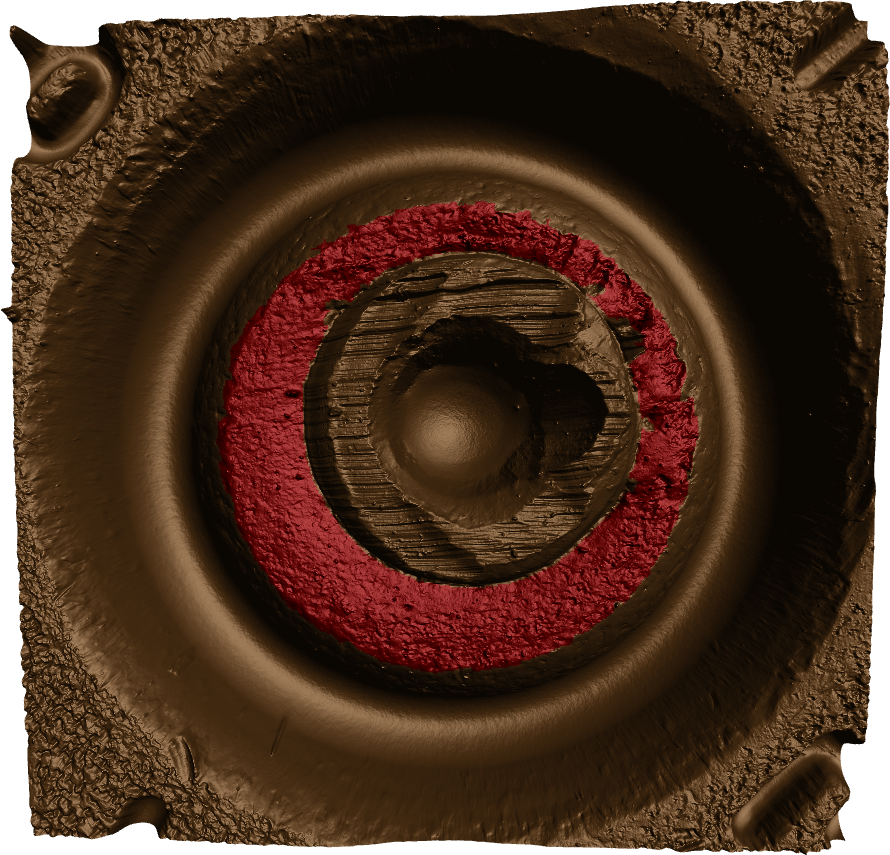
\includegraphics[width=.6\textwidth]{images/annotatedReference} 

}

\caption{\label{fig:annotatedScan} A cartridge case surface is manually annotated in red using the FiX3P software. The annotated region of interest contains breech face impressions.}\label{fig:unnamed-chunk-1}
\end{figure}
\end{CodeChunk}

Once read into an R environment, we use sequence of functions available
in the {[}x3ptools{]} and {[}cmcR{]} packages to preprocess the raw
scans. \autoref{fig:preProcessEffect} shows the effect that each
function has on the scan surface values. Gray pixels in each plot
represent missing values in the surface matrix. The \texttt{x3p\_delete}
function removes values in the scan based on the associated mask. Next,
the \texttt{preProcess\_removeTrend} function subtracts a fitted
conditional median plane from the surface values to ``level-out'' any
global tilt in the scan. The \texttt{preProcess\_gaussFilter()} function
applies a bandpass Gaussian filter to remove small-scale noise and other
large-scale structure, which better highlights the medium-scale breech
face impressions. Finally, the \texttt{preProcess\_erode()} function
applies the morphological operation of erosion on the edge of the
non-missing surface values {[}cite erosion reference{]}. This has the
effect of shaving-off values on the interior and exterior edge of the
surface, which are often extreme ``roll-off'' values that unduly affect
the comparing stage if not removed. The final result is a cartridge case
surface matrix with emphasized breech face impressions.

\begin{CodeChunk}
\begin{figure}[htbp]

{\centering 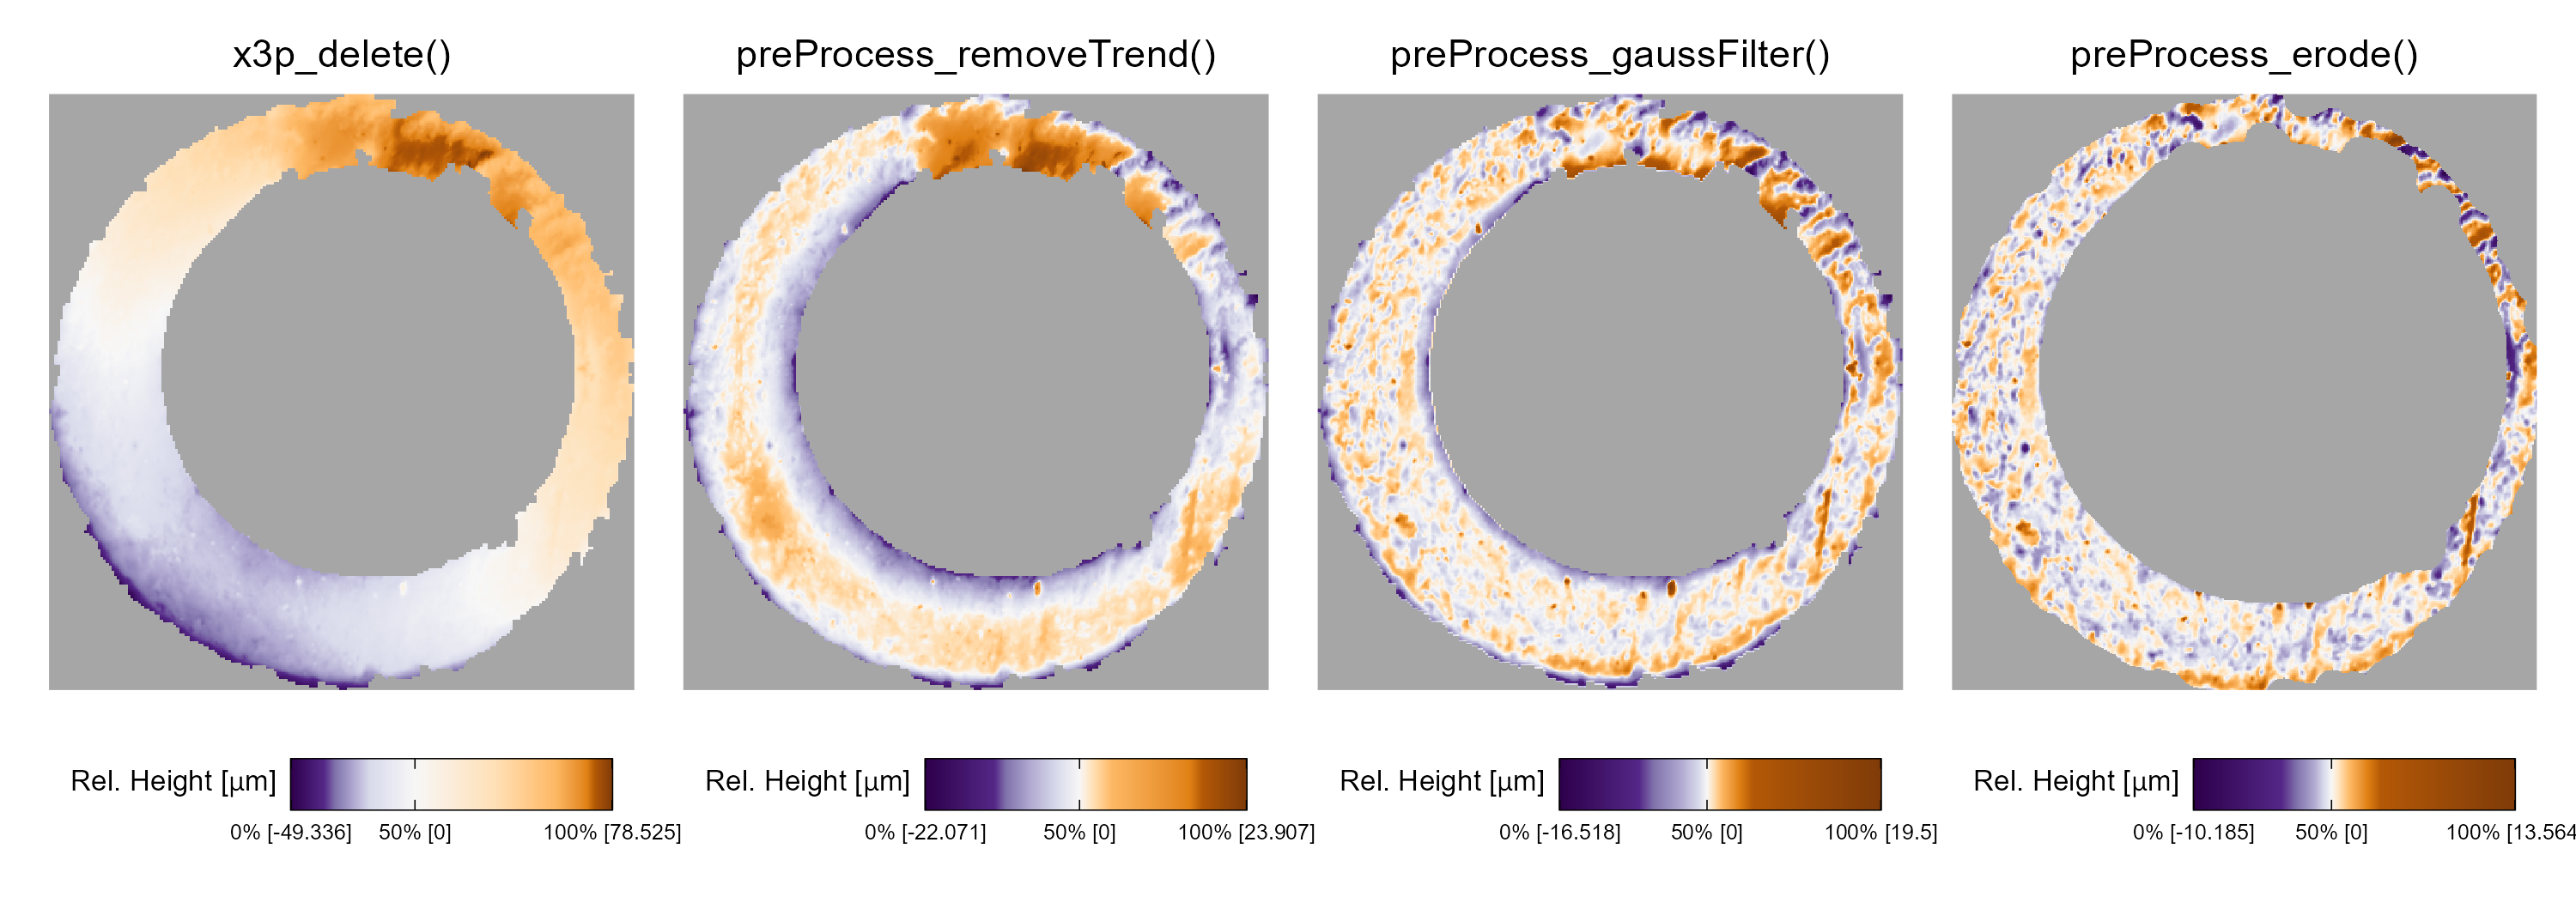
\includegraphics[width=\textwidth]{figures/preProcessEffect} 

}

\caption{\label{fig:preProcessEffect} We apply a sequence of preprocessing functions to each scan. Each preprocessing step further emphasizes the breech face impressions in the scan.}\label{fig:unnamed-chunk-4}
\end{figure}
\end{CodeChunk}

Next, we compute a set of similarity features for two preprocessed
cartridge case scans.

\hypertarget{comparing}{%
\subsection{Comparing}\label{comparing}}

In this section, we introduce a set of similarity features for two
cartridge case scans. We calculate features at two scales: between two
whole scans and between individual cells similar to the CMC method
{[}cite{]}. Analogous to how a forensic examiner uses a comparison
microscope with different magnification levels, this allows us to assess
the similarity between two scans at the macro and micro levels.

\hypertarget{notational-conventions}{%
\subsubsection{Notational Conventions}\label{notational-conventions}}

First, we introduce notation that will be used to define the features.
Let \(A\) and \(B\) denote two surfaces matrices that we wish to
compare. For simplicity, we assume that
\(A,B \in \mathbb{R}^{k \times k}\) for
\(k > 0\).\footnote{This assumption of equally-sized, square matrices is easily enforced by padding the matrices with additional missing values.
Due to the presence of (structurally) missing values around the breech face impression region, additional padding does not interfere with the structure of the scan.}
We use lowercase letters and subscripts to denote a particular value of
a matrix: \(a_{ij}\) is the value in the \(i\)th row and \(j\)th column,
starting from the top-left corner, of matrix \(A\). Throughout this
section, we will use the two known-match cartridge cases in
\autoref{fig:matchPair} as exemplar matrices \(A\) and \(B\).

To accommodate structurally-missing values, we adapt standard matrix
algebra as follows: if an element of either matrix \(A\) or \(B\) is
missing, then any element-wise operation including this element is also
missing, otherwise standard matrix algebra holds. For example, the
addition operator is defined as: \begin{align*}
A \oplus_{NA} B = (a_{ij} \oplus_{NA} b_{ij})_{1 \leq i,j \leq k} = 
\begin{cases}
a_{ij} + b_{ij} & \text{if both $a_{ij}$ and $b_{ij}$ are numbers} \\
NA &\text{otherwise}
\end{cases}
\end{align*} Other element-wise operations such as \(\ominus_{NA}\) are
defined similarly. For readability, we will use standard operator
notation \(+, -, >, <, ...\) and assume the extended operations as
defined above.

\begin{CodeChunk}
\begin{figure}[htbp]

{\centering 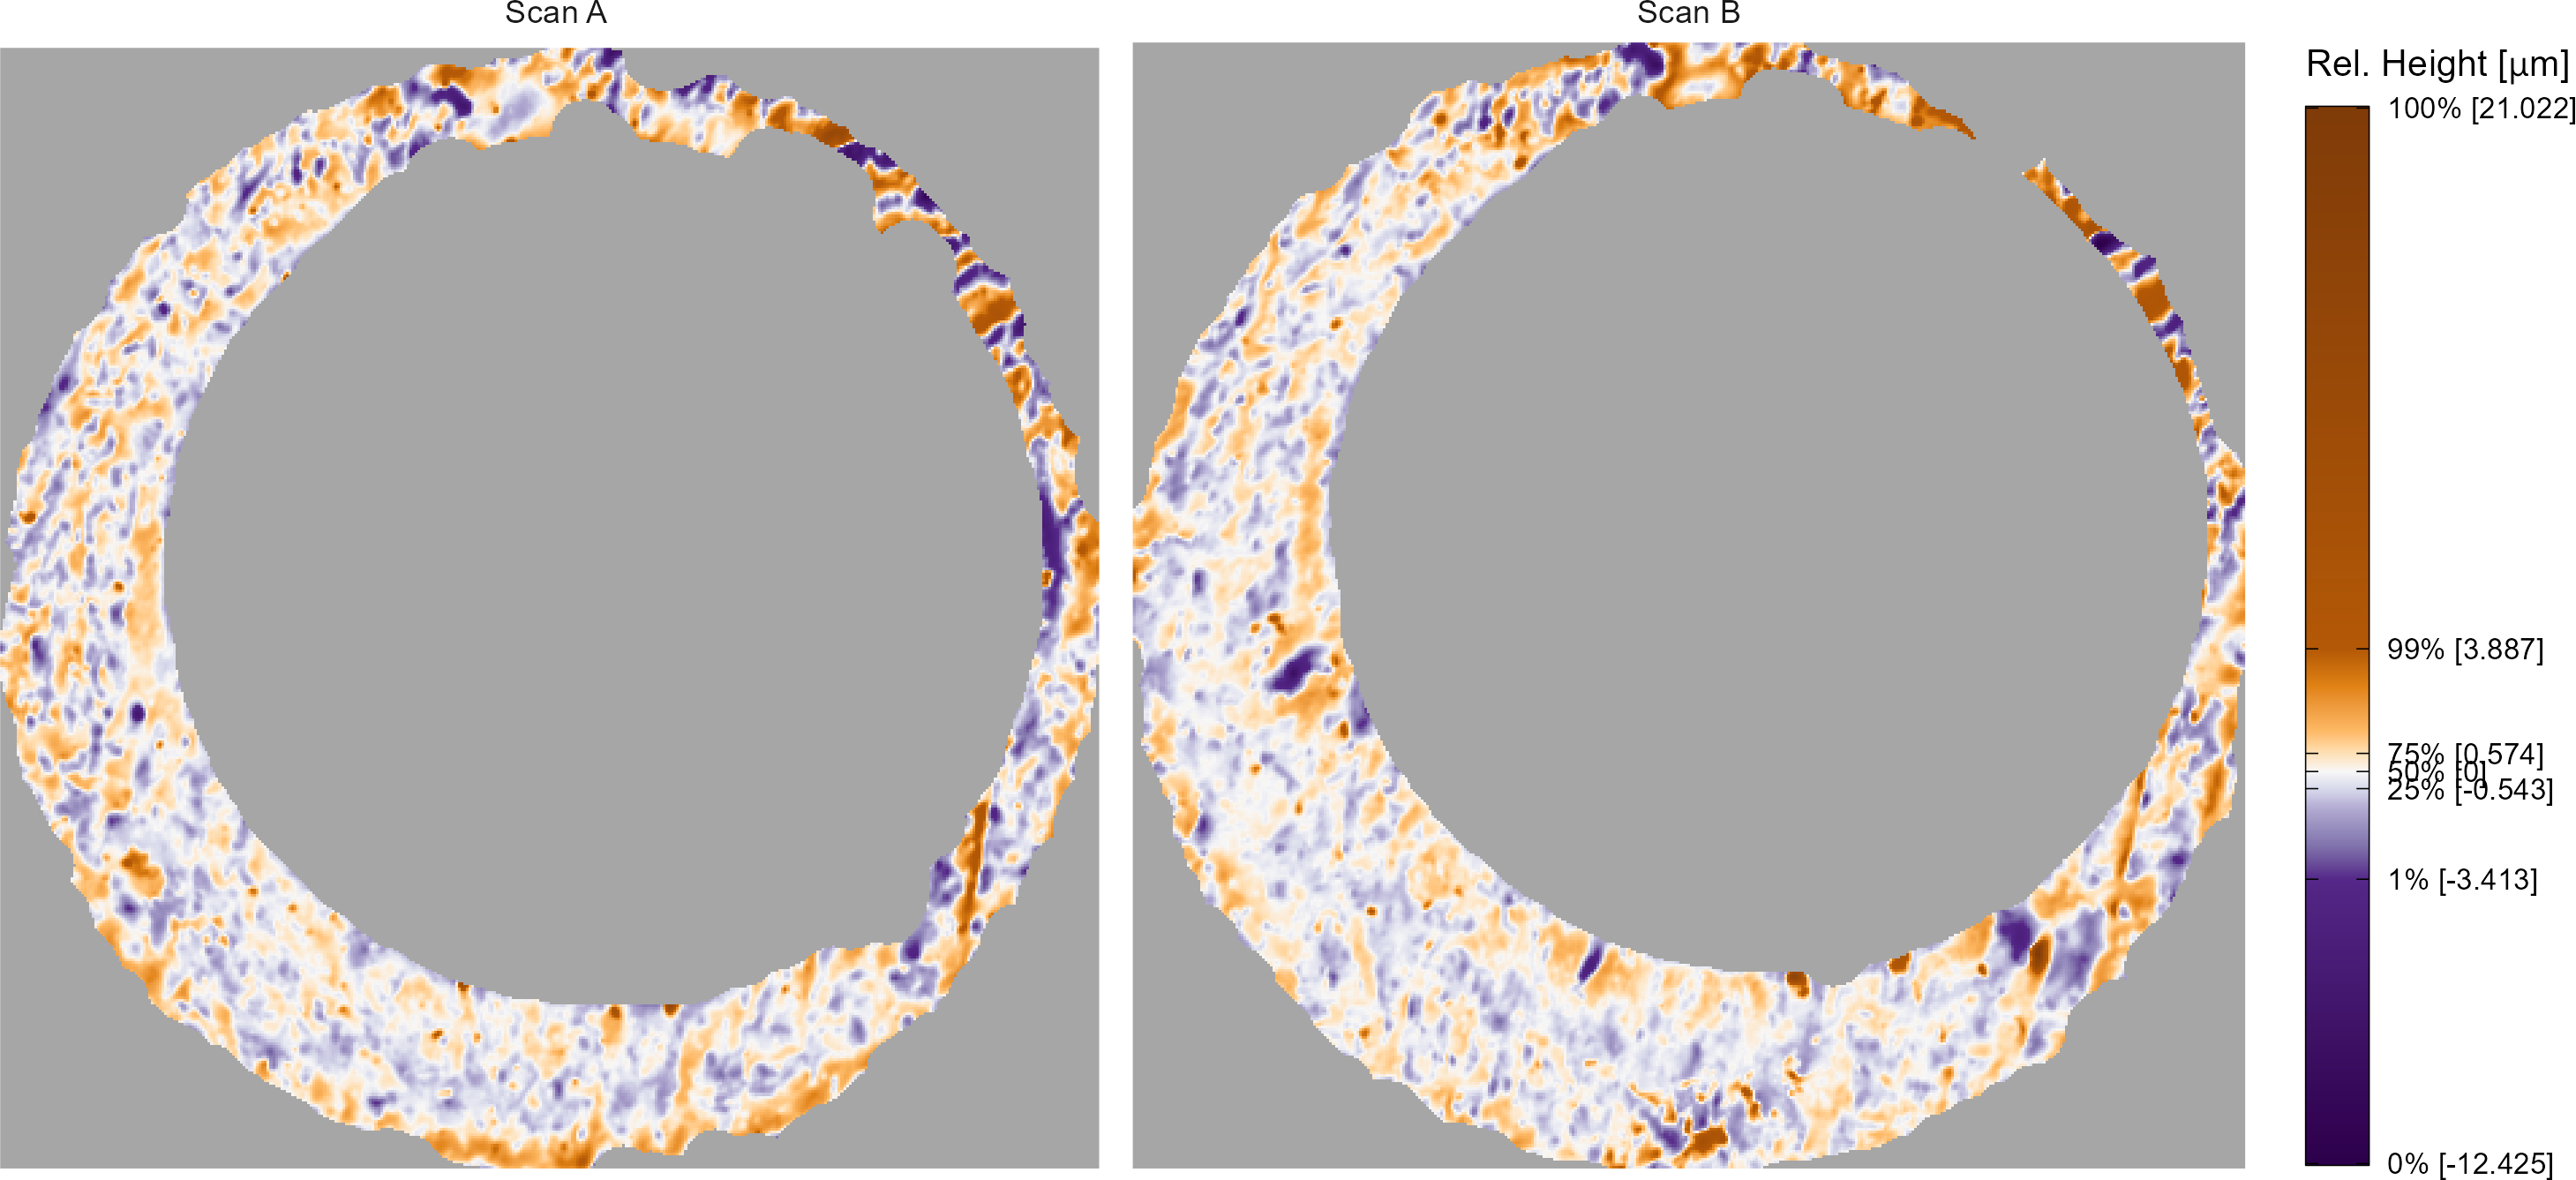
\includegraphics[width=\textwidth]{figures/matchPair} 

}

\caption{\label{fig:matchPair} A matching pair of processed cartridge case scans. We measure the similarity between these cartridge cases using the distinguishable breech face impressions on their surfaces.}\label{fig:unnamed-chunk-6}
\end{figure}
\end{CodeChunk}

\hypertarget{registration-estimation}{%
\subsubsection{Registration Estimation}\label{registration-estimation}}

A critical step in comparing \(A\) and \(B\) is to find a transformation
of \(B\) such that it aligns best to \(A\) (or vice versa). In image
processing, this is called \emph{image registration.} Noting that \(A\)
and \(B\) are essentially grayscale images, we rely on a standard image
registration technique {[}cite Brown, 1992{]}.

In our application, a registration is composed of a discrete translation
by \((m,n) \in \mathbb{Z}^2\) and rotation by
\(\theta \in [-180^\circ,180^\circ]\). Under this transformation, the
index \(i,j\) maps to a new index \(i^*,j^*\) by: \begin{align*}
\begin{pmatrix} j^* \\ i^* \end{pmatrix} =
\begin{pmatrix} n \\ m \end{pmatrix} +
\begin{pmatrix} \cos(\theta) & -\sin(\theta) \\ \sin(\theta) & \cos(\theta) \end{pmatrix} \begin{pmatrix} j \\ i \end{pmatrix}.
\end{align*}

The value \(b_{ij}\) now occupies the index \(i^*, j^*\). In practice,
we use \emph{nearest-neighbor interpolation} meaning \(i^*\) and \(j^*\)
are rounded to the nearest integer {[}cite a nearest-neighbor
reference{]}.

To determine the optimal registration, we calculate the
\emph{cross-correlation function} (CCF) between \(A\) and \(B\), which
measures the similarity between \(A\) and \(B\) for every possible
translation of \(B\). Denoted \((A \star B)\), the CCF between \(A\) and
\(B\) is a 2D array of dimension \(2k - 1 \times 2k - 1\) with the
\(m,n\)-th element given by: \begin{align*}
(a \star b)_{mn} = \sum_{i=1}^k \sum_{j=1}^k a_{mn} \cdot b_{i + m, j + n}
\end{align*} where \(1 \leq m,n \leq 2k - 1\). The value
\((a \star b)_{mn}\) quantifies the similarity between \(A\) and \(B\)
after \(B\) is translated \(m\) elements horizontally and \(n\) elements
vertically. The CCF is often normalized between -1 and 1 for
interpretability.

For large matrices, the above definition of the CCF is computationally
taxing. The Cross-Correlation Theorem provides an equivalent expression
for the CCF: \begin{align*}
(A \star B) = \mathcal{F}^{-1}\left(\overline{\mathcal{F}(A)} \odot \mathcal{F}(B)\right)
\end{align*} where \(\mathcal{F}\) and \(\mathcal{F}^{-1}\) are the
discrete Fourier and inverse discrete Fourier transforms, respectively,
\(\overline{\mathcal{F}(A)}\) is the complex conjugate, and \(\odot\) is
an element-wise (Hadamard) product {[}cite Brigham, 1988{]}. We trade
the moving sum computation from the previous CCF expression for two
forward Fourier transforms, an element-wise product, and an inverse
Fourier transform. The Fast Fourier Transform (FFT) algorithm reduces
the computational load considerably {[}cite Tukey{]}.

Using the CCF as an objective function, we estimate the registration by
calculating the maximum CCF value across a range of rotations of matrix
\(B\). Let \(B_\theta\) denote \(B\) rotated by an angle
\(\theta \in [-180^\circ,180^\circ]\) and \(b_{\theta_{mn}}\) the
\(m,n\)-th element of \(B_\theta\). Then the estimated registration
\((m^*,n^*,\theta^*)\) is: \begin{align*}
(m^*,n^*,\theta^*) = \arg \max_{m,n,\theta} (a \star b_\theta)_{mn}.
\end{align*} In practice we consider a discrete grid of rotations
\(\pmb{\Theta} \subset [-180^\circ,180^\circ]\). The registration
procedure is outlined in \autoref{alg:registration}. We refer to the
matrix that is rotated as the ``target.'' The result is the estimated
registration of the target matrix to the ``source'' matrix.

\begin{algorithm}[htbp]
\KwData{Source matrix $A$, target matrix $B$, and rotation grid $\pmb{\Theta}$}
\KwResult{Estimated registration of $B$ to $A$, $(m^*,n^*,\theta^*)$, and cross-correlation function maximum, $CCF_{\max}$}
\For{$\theta \in \pmb{\Theta}$}{
Rotate $B$ by $\theta$ to obtain $B_\theta$\;
Calculate $CCF_{\max, \theta} = \max_{m,n} (a \star b_{\theta})_{mn}$\;
Calculate translation $[m^*_\theta,n^*_\theta] = \arg \max_{m,n} (a \star b_{\theta})_{mn}$
}
Calculate overall maximum correlation $CCF_{\max} = \max_{\theta} \{CCF_{\max,\theta} : \theta \in \pmb{\Theta}\}$\;
Calculate rotation $\theta^* = \arg \max_{\theta} \{CCF_{\max,\theta} : \theta \in \pmb{\Theta}\}$\;
\Return{Estimated rotation $\theta^*$, translation $m^* = m^*_{\theta^*}$ and $n^* = n^*_{\theta^*}$, and $CCF_{\max}$}
\caption{Image Registration Procedure}
\label{alg:registration}
\end{algorithm}

\hypertarget{handling-missingness}{%
\subsubsection{Handling Missingness}\label{handling-missingness}}

\textbf{[Not sure what to do with this section.
It needs to be mentioned, but in more or less detail?]}

The registration estimation procedure outline above, namely the Fast
Fourier Transform algorithm, does not permit missing values in \(A\) or
\(B\). It is common for cartridge case scans to contain many missing
values - the gray regions in {[}preprocessing Figure{]} represent
structural values in the scan. Thus, when calculating the CCF we impute
these missing values with the average non-missing value in the scan.

We wish to measure the similarity between \(A\) and \(B\) while taking
this missingness into account; to measure the similarity between the
non-missing intersection of the aligned scans. We compute the
\emph{pairwise-complete correlation} using only the complete value
pairs, meaning neither value is missing, between \(A\) and \(B\).

\hypertarget{registration-based-features}{%
\subsubsection{Registration-Based
Features}\label{registration-based-features}}

\hypertarget{full-scan-registration}{%
\paragraph{Full-Scan Registration}\label{full-scan-registration}}

We first estimate the registration between two full scans \(A\) and
\(B\) using \autoref{alg:registration} with a rotation grid
\(\pmb{\Theta} = \{-30^\circ, -27^\circ,...,27^\circ,30^\circ\}\). This
results in an estimated registration \((m^*,n^*,\theta^*)\) and
similarity measure \(CCF_{\max}\). We also perform
\autoref{alg:registration} with the roles of \(A\) and \(B\) reversed,
meaning the target scan \(A\) is aligned to source scan \(B\) to obtain
\(A^*\).

To accommodate these two comparison directions, we introduce a new
subscript \(d = A,B\), referring to the source scan in
\autoref{alg:registration}. Consequently, we obtain two sets of sets of
estimated registrations, \((m^*_d,n^*_d,\theta^*_d)\) and
\(CCF_{\max,d}\) for
\(d=A,B\).\footnote{In reality, the true aligning registrations in the two comparison directions are opposites of each other. However, because we compare discretely-indexed arrays using a nearest-neighbor interpolation scheme, the estimated registrations differ slightly.}
For \(d = A\), we then apply the registration transformation
\((m^*_A,n^*_A,\theta^*_A)\) to \(B\) to obtain \(B^*\) and compute the
pairwise-complete correlation, \(cor_{\text{full},A}\), between \(A\)
and \(B^*\). We repeat this in the other comparison direction to obtain
\(cor_{\text{full},B}\) and average the two: \begin{align*}
cor_{\text{full}} = \frac{1}{2}\left(cor_{A,\text{full}} + cor_{B,\text{full}}\right).
\end{align*} We assume that the \textbf{average full-scan
pairwise-complete correlation} is large for truly matching cartridge
cases.

\hypertarget{cell-based-registration}{%
\paragraph{Cell-Based Registration}\label{cell-based-registration}}

Following the full-scan registration, we next perform a cell-based
registration procedure. {[}Song (2013){]} points out that breech face
impressions rarely appear uniformly on a cartridge case surface. Rather,
distinguishing markings appear in specific, usually small, regions of a
scan (the author refers to these as \emph{valid correlation regions}).
Calculating a correlation between two whole scans does not necessarily
capture the similarity between these regions. {[}Song (2013){]} proposes
partitioning a scan into a rectangular grid of ``cells'' to isolate the
valid correlation regions. \autoref{fig:cellGridExample} shows an
example of matrix \(A\) partitioned into a grid of \(8 \times 8\) cells.

\begin{CodeChunk}
\begin{figure}[htbp]

{\centering 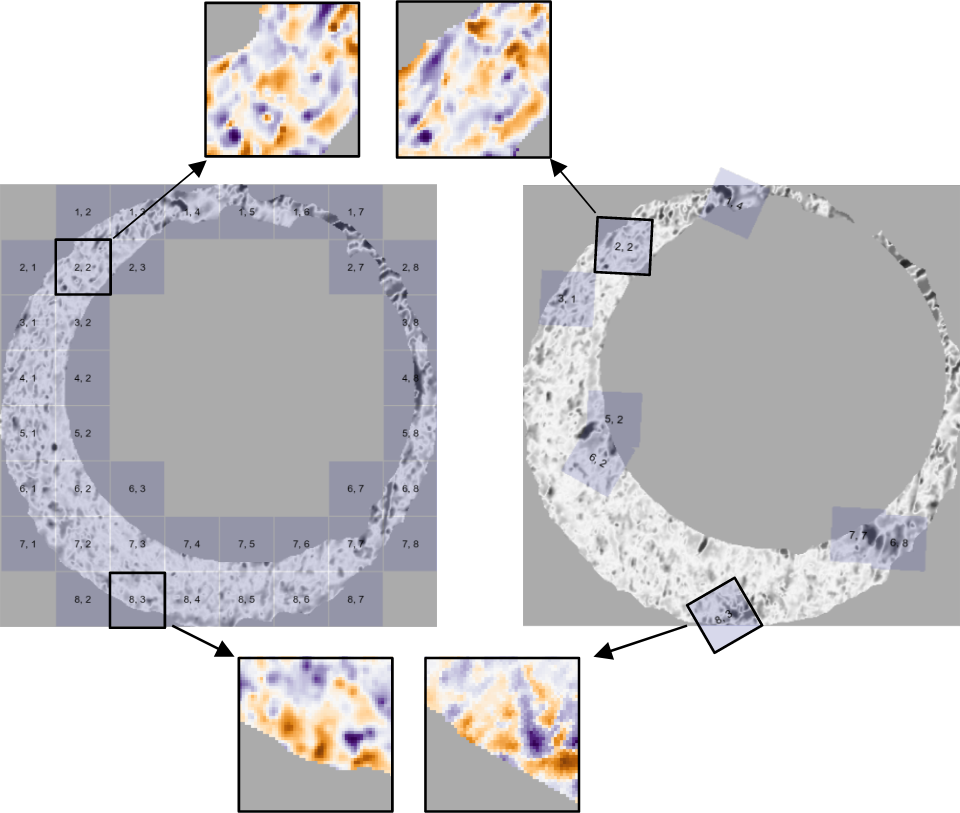
\includegraphics[width=\textwidth]{images/cellGridExample} 

}

\caption{\label{fig:cellGridExample} A source scan separated into a grid of $8 \times 8$ cells. Each source cell is compared to a target scan to estimate where it aligns best. We exclude cells containing only missing values (visualized here as gray pixels).}\label{fig:unnamed-chunk-7}
\end{figure}
\end{CodeChunk}

The cell-based comparison procedure begins with selecting one of the
matrices, say \(A\), as the ``source'' matrix to be partitioned into a
grid of cells. Each of these source cells will be compared to the
``target'' matrix, in this case \(B^*\). Because \(A\) and \(B^*\) are
already partially aligned based on the course rotation grid
\(\pmb{\Theta}\), we compare each source cell to \(B^*\) using a new
rotation grid of
\(\pmb{\Theta}'_A = \{\theta^*_A - 2^\circ, \theta^*_A - 1^\circ,\theta^*_A,\theta^*_A + 1^\circ,\theta^*_A + 2^\circ\}\).

We now extend the surface matrix notation introduced previously to
accommodate cells. Let \(A_{t}\) denote the \(t\)th cell of matrix
\(A\), \(t = 1,...,T_A\) where \(T_A\) is the total number of cells
containing non-missing values (e.g., \(T_A = 38\) in
\autoref{fig:cellGridExample}) in scan \(A\) and let \((a_t)_{ij}\)
denote the \(i,j\)-th element of \(A_t\).

The cell-based comparison procedure is outlined in
\autoref{alg:cellComparison}.

\begin{algorithm}[H]
\KwData{Source matrix $A$, target matrix $B^*$, cell grid size $R \times C$, and rotation grid $\pmb{\Theta}'_A$}
\KwResult{Estimated translations and $CCF_{\max}$ values per cell, per rotation}
Partition $A$ into a grid of $R \times C$ cells\;
Discard cells containing only missing values, leaving $T_A$ remaining cells\;
\For{$\theta \in \pmb{\Theta}'_A$}{
Rotate $B^*$ by $\theta$ to obtain $B^*_\theta$\;
\For{$t = 1,...,T_A$}{
Calculate $CCF_{\max, A,t,\theta} = \max_{m,n} (a_t \star b^*_\theta)_{mn}$\;
Calculate translation $[m^*_{A,t,\theta},n^*_{A,t,\theta}] = \arg \max_{m,n} (a_t \star b^*_\theta)_{mn}$
}
}
\Return{$\pmb{F}_A = \{(m^*_{A,t,\theta},n^*_{A,t,\theta}, CCF_{\max,A,t,\theta}, \theta) : \theta \in \pmb{\Theta}'_A, t = 1,...,T_A\}$}
\caption{Cell-Based Comparison Procedure}
\label{alg:cellComparison}
\end{algorithm}

Rather than exclusively returning the registration that maximizes the
overall CCF as in \autoref{alg:registration},
\autoref{alg:cellComparison} returns the set \(\pmb{F}_A\) of
translations and CCF values for each cell and each rotation considered.
If two cartridge cases are truly matching, then we assume that multiple
cells will ``agree'' on a particular translation value at the true
rotation.\footnote{And that cells will not come to such an agreement for a non-matching pair of cartridge cases}
This agreement phenomenon is illustrated in
\autoref{fig:estimatedTranslationFaceted} where each point represents
the translation that maximizes the CCF for a particular cell and
rotation. The points appear randomly distributed for most of the
rotation values except around \(\theta = 3\) where a tight cluster of
points forms around translation \([17,-16]\). This is evidence to
suggest that a true registration exists for these two cartridge cases,
implying that they match. The task is to determine when cells reach a
registration consensus.

\begin{CodeChunk}
\begin{figure}[htbp]

{\centering 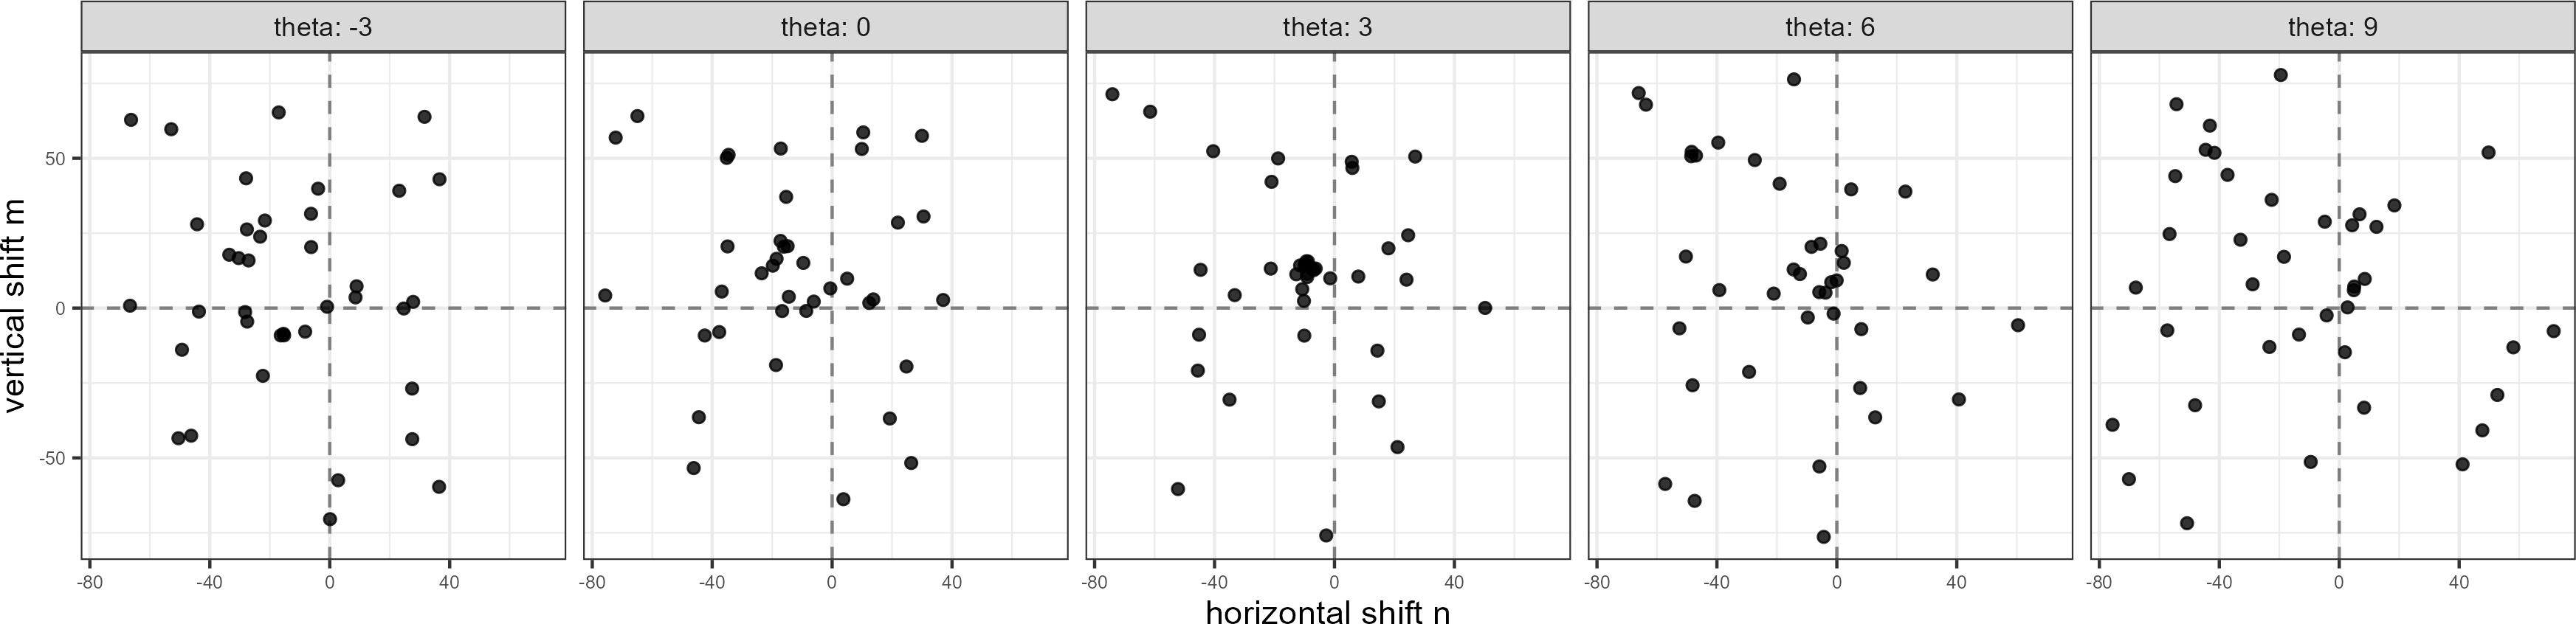
\includegraphics[width=\textwidth]{figures/estimatedTranslationFaceted} 

}

\caption{\label{fig:estimatedTranslationFaceted} A scatterplot where points represent the cell-wise estimated translations faceted by rotation for a matching pair of cartridge cases. As evidenced by the tight cluster in the middle facet, it appears that multiple cells agree on a translation of $[\hat{m}, \hat{n}] \approx  [17,-16]$ after rotating by $3^\circ$. Points are jittered for visibility.}\label{fig:unnamed-chunk-10}
\end{figure}
\end{CodeChunk}

Just as with the whole-scan registration, we calculate the
pairwise-complete correlation between each cell \(A_t\) and a matrix
\(B_{\theta,t}^*\) of the same size extracted from \(B^*_{\theta}\)
after translating by \([m^*_{A,\theta},n^*_{A,\theta}]\). From this we
obtain a set of pairwise-complete correlations for each rotation:
\(\{cor_{A,t,\theta} : \theta \in \pmb{\Theta}'_A\}\). This whole
procedure is repeated using \(B\) as the source scan and \(A^*\) as the
target, resulting in registration set \(\pmb{F}_B\) and
pairwise-complete correlations
\(\{cor_{B,t,\theta} : \theta \in \pmb{\Theta}'_B\}\).

For \(d = A,B\) and \(t = 1,...,T_d\), define the cell-wise maximum CCF
and pairwise-complete correlation as: \begin{align*}
CCF_{\max,d,t} &= \max_{\theta} \{CCF_{\max,d,t,\theta} : \theta \in \pmb{\Theta}'_d\} \\
cor_{d,t} &= \max_{\theta} \{cor_{d,t,\theta} : \theta \in \pmb{\Theta}'_d\}
\end{align*}

We compute the \textbf{average} and
\textbf{standard deviation of the cell-based pairwise-complete correlations}
features using the correlation data: \begin{align*}
\overline{cor}_{\text{cell}} &= \frac{1}{T_A + T_B} \sum_{d \in \{A,B\}} \sum_{t=1}^{T_d} cor_{d,t} \\
s_{cor} &= \sqrt{\frac{1}{T_A + T_B - 1} \sum_{d \in \{A,B\}} \sum_{t=1}^{T_d} (cor_{d,t} - \overline{cor}_{\text{cell}})^2}
\end{align*}

We expect the \(\overline{cor}_{\text{cell}}\) to be large and the
\(s_{cor}\) small for truly matching cartridge case pairs.

For \(d = A,B\) and \(t = 1,...,T_d\), define the per-cell estimated
translations and rotation as: \begin{align*}
\theta^*_{d,t} &= \arg \max_{\theta} \{CCF_{\max,d,t,\theta} : \theta \in \pmb{\Theta}'_d\} \\
m^*_{d,t} &= m^*_{\theta^*_{d,t},d,t} \\
n^*_{d,t} &= n^*_{\theta^*_{d,t},d,t}
\end{align*}

We compute the
\textbf{standard deviation of the cell-based estimated registration}
using the estimated cell translations and rotations: \begin{align*}
s_{\theta^*} =  \sqrt{\frac{1}{T_A + T_B - 1} \sum_{d \in \{A,B\}} \sum_{t=1}^{T_d} (\theta^*_{d,t} - \bar{\theta}^*)^2} \\
s_{m^*} =  \sqrt{\frac{1}{T_A + T_B - 1} \sum_{d \in \{A,B\}} \sum_{t=1}^{T_d} (m^*_{d,t} - \bar{m}^*)^2} \\
s_{n^*} = \sqrt{\frac{1}{T_A + T_B - 1} \sum_{d \in \{A,B\}} \sum_{t=1}^{T_d} (n^*_{d,t} - \bar{n}^*)^2}
\end{align*} where \begin{align*}
\bar{m}^* &= \frac{1}{T_A + T_B} \sum_{d \in \{A,B\}}\sum_{t=1}^{T_d} m^*_{d,t} \\
\bar{n}^* &= \frac{1}{T_A + T_B} \sum_{d \in \{A,B\}} \sum_{t=1}^{T_d} n^*_{d,t} \\
\bar{\theta}^* &= \frac{1}{T_A + T_B} \sum_{d \in \{A,B\}} \sum_{t=1}^{T_d} \theta^*_{d,t}.
\end{align*} We expect the \(s_{\theta^*}, s_{m^*},s_{n^*}\) to be small
for truly matching cartridge case pairs.

\autoref{fig:registrationDensities} shows density plots of the
registration-based features for 21,945 cartridge case pairs. The first
two rows show densities for the sample mean and standard deviation of
the cell-based registrations, respectively. The third row shows
densities for the pairwise-complete correlation features. The standard
deviation of the cell-based registrations discriminate more between
match vs.~non-match pairs than the sample means, which justifies their
exclusion from the final feature set. {[}More to say here?{]}

\begin{CodeChunk}
\begin{figure}[htbp]

{\centering 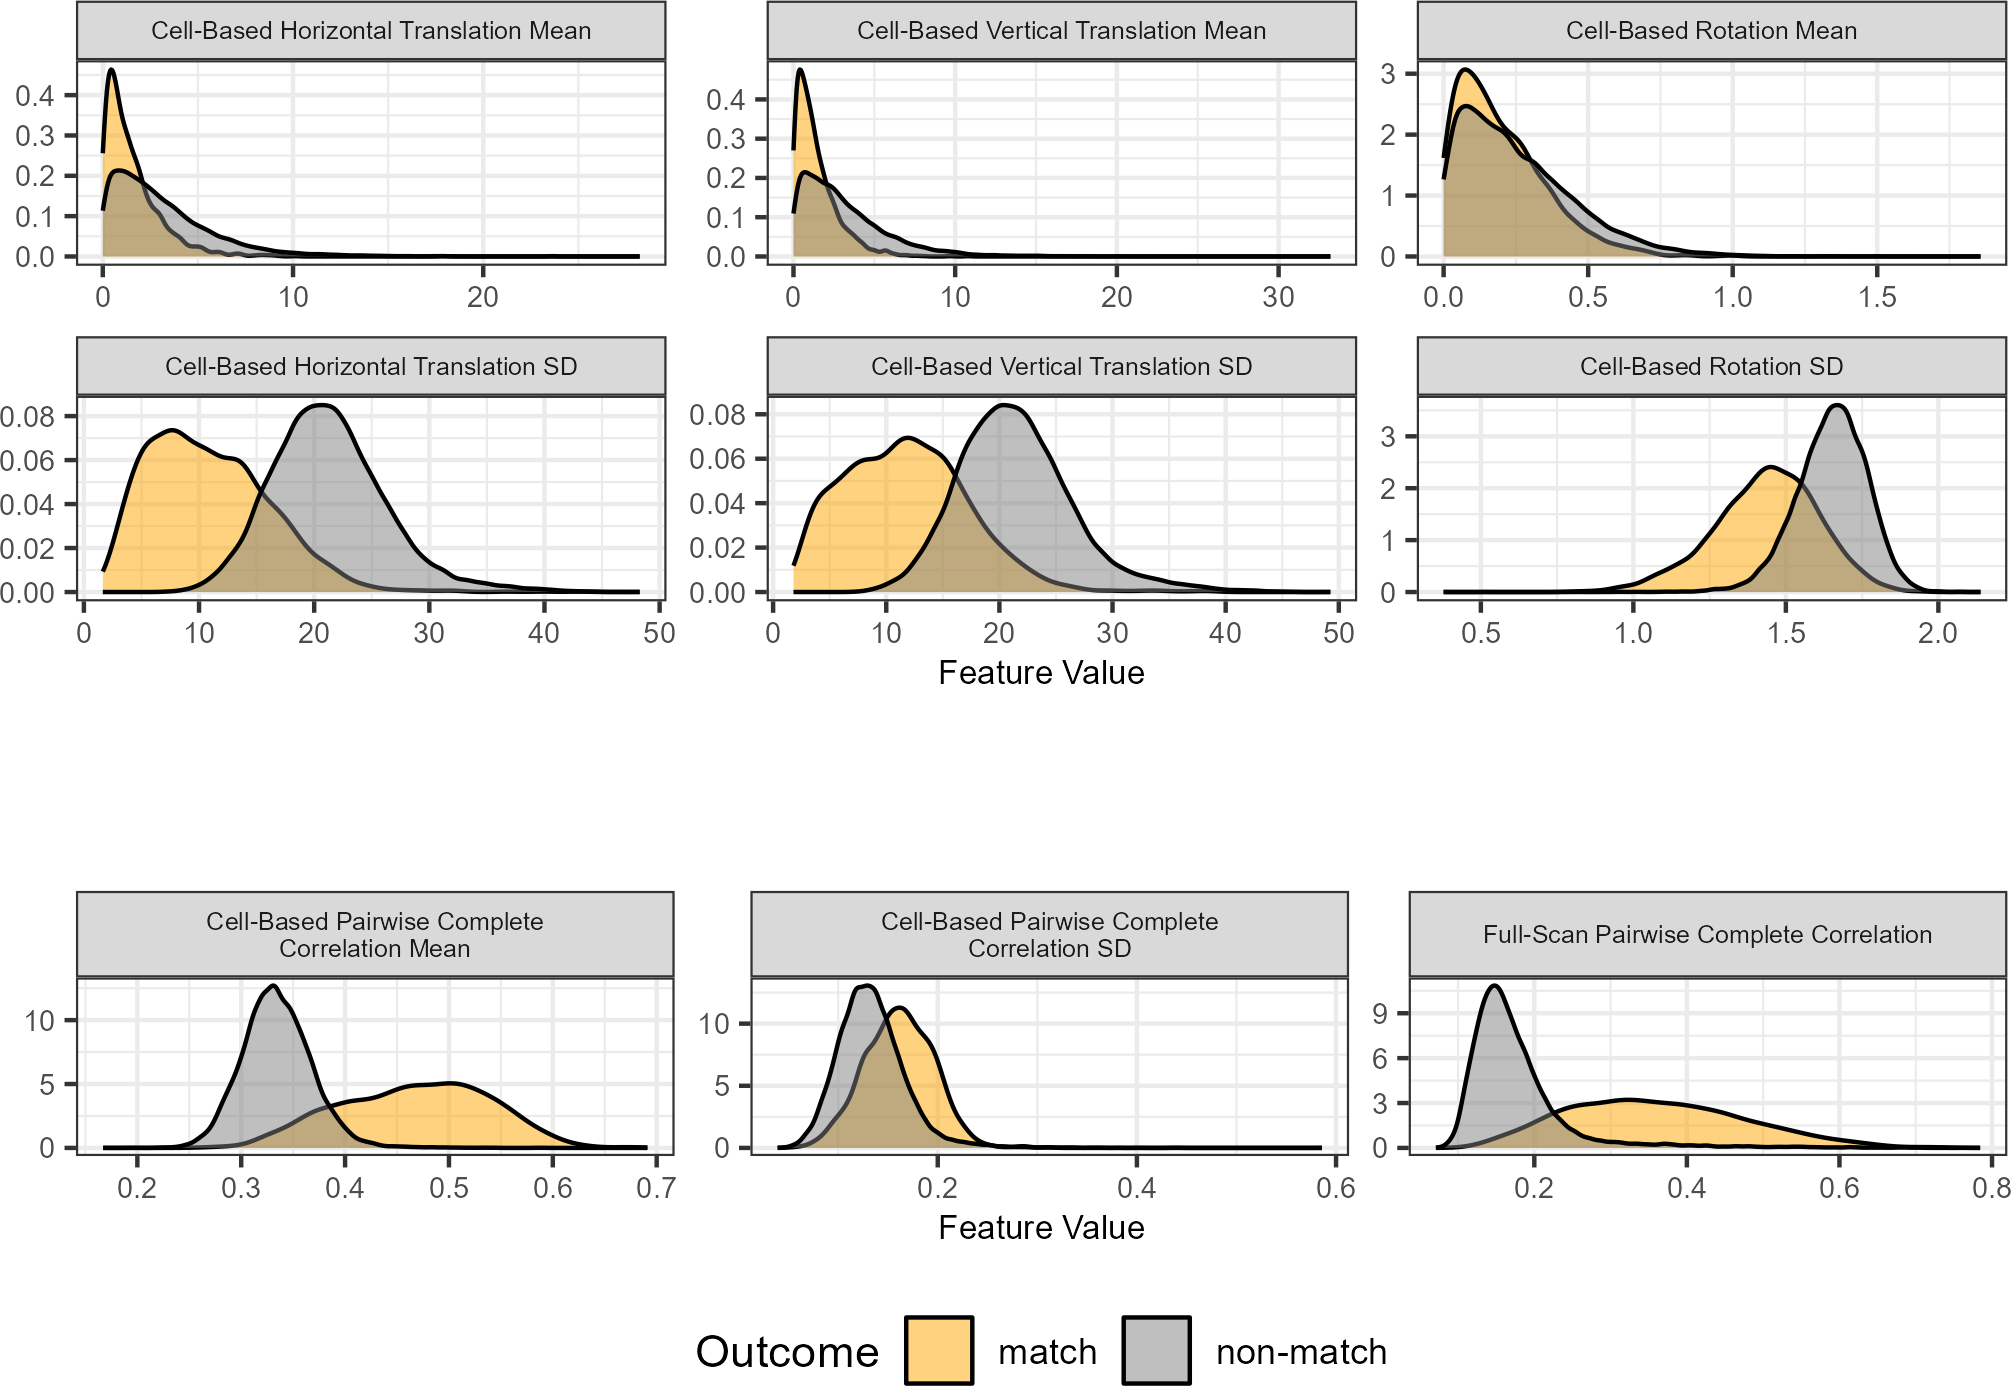
\includegraphics[width=\textwidth]{images/registrationFeatureDensities} 

}

\caption{\label{fig:registrationDensities} Density plots of the Registration-Based features for 21,945 cartridge case pairs. The standard deviation of the cell-based registrations distinguish between match and non-match pairs better than the mean values.}\label{fig:unnamed-chunk-11}
\end{figure}
\end{CodeChunk}

From the full-scan and cell-based registration procedures, we obtain six
features summarized in \autoref{tab:registrationFeatures}.

\begin{table}[htbp]
\centering
\begin{tabular}{|p{.11\linewidth}|p{.7\linewidth}|}
\hline
Notation & Feature Description \\
\hline
$cor_{\text{full}}$ & \textbf{Full-scan pairwise-complete correlation} after aligning the scans. \\
\hline
$\overline{cor}_{\text{cell}}$ & \textbf{Average cell-based pairwise-complete correlation} after aligning source cells to the target matrix using the cross-correlation function \\
\hline
$s_{cor}$ & \textbf{Standard deviation of the cell-based pairwise-complete correlation} after aligning source cells to the target matrix using the cross-correlation function \\
\hline
$s_{m^*}$ & \textbf{Standard deviation of the cell-based vertical translations} \\
\hline
$s_{n^*}$ & \textbf{Standard deviation of the cell-based horizontal translations} \\
\hline
$s_{\theta^*}$ & \textbf{Standard deviation of the cell-based rotations} \\
\hline
\end{tabular}
\caption{Six similarity features based on registering full scans or cells.}
\label{tab:registrationFeatures}
\end{table}

\hypertarget{density-based-features}{%
\subsubsection{Density-Based Features}\label{density-based-features}}

As discussed in the last section, we wish to identify when multiple
cells agree on a particular registration. {[}Zhang et al.~(2020){]}
proposed using the Density-Based Spatial Clustering of Applications with
Noise (DBSCAN) algorithm to identify clusters of points based on their
density.

\autoref{fig:dbscanIllustration} depicts an illustration of the DBSCAN
algorithm {[}cite Wikimedia commons{]}. The algorithm has two
parameters: a neighborhood radius \(\epsilon\) and a minimum point
threshold \(Minpts\). In \autoref{fig:dbscanIllustration},
\(Minpts = 4\) and \(\epsilon\) is arbitrary and represented by the
radius of the circles drawn around each point - each circle represents
the \(\epsilon\)-neighborhood for its center point. First, the algorithm
identifies cluster ``core'' points that contain at least \(Minpts\)
points within an \(\epsilon\)
distance.\footnote{Euclidean distance, in our application} These points
form the beginning of a cluster and are shown in red in
\autoref{fig:dbscanIllustration}. The yellow points \(B\) and \(C\) are
within the \(\epsilon\)-neighborhood of a core point, but are not
themselves core points. They are also included in the cluster making the
overall cluster size 8. Finally, the blue point labelled \(N\) is not in
any core point's \(\epsilon\)-neighborhood and is thus classified as a
``noise point.'' Unlike other clustering algorithms, the DBSCAN
algorithm does not require a specified number of expected clusters as a
parameter; any points not belonging to a cluster are ``noise.''

\begin{CodeChunk}
\begin{figure}[htbp]

{\centering 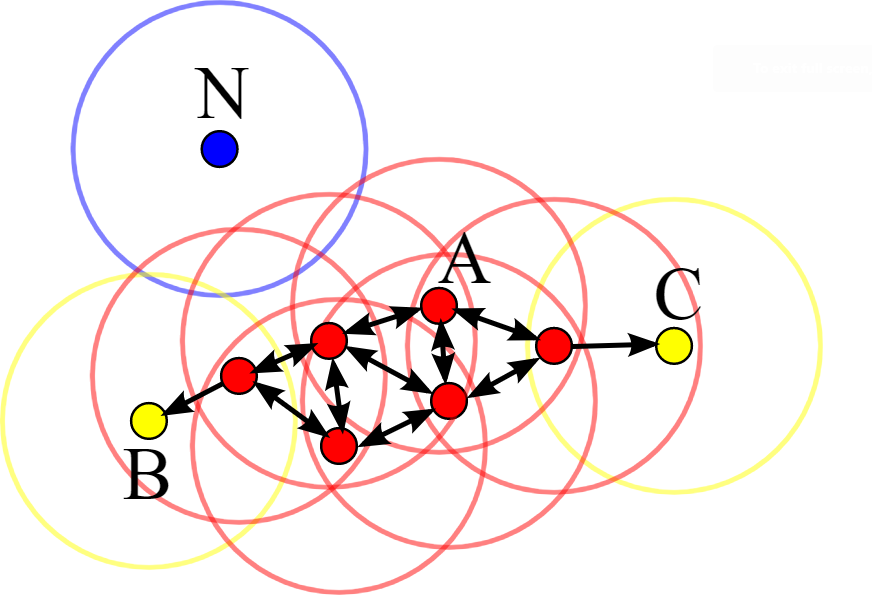
\includegraphics[width=.7\textwidth]{images/dbscanIllustration} 

}

\caption{\label{fig:dbscanIllustration} Illustration of the DBSCAN algorithm [cite]. Red and yellow points are part of the same cluster with the former forming the "core" of the cluster. The blue point is not part of a cluster and is classified as a "noise point." Figure by Chire - Own work, CC BY-SA 3.0, https://commons.wikimedia.org/w/index.php?curid=17045963}\label{fig:unnamed-chunk-12}
\end{figure}
\end{CodeChunk}

\autoref{fig:dbscanScatterplot} shows an example of DBSCAN cluster
assignments for the known-match pair \(A\) and \(B\) shown in
\autoref{fig:matchPair}. The left scatterplot shows the per-cell
estimated translations \([m^*_{d,t,\theta}, n^*_{d,t,\theta}]\) for
\(\theta = 3^\circ\) when scan \(A\) is used as source and \(B^*\) as
target, resulting a cluster of size 14. The right scatterplot shows the
per-cell estimated translations with the roles of \(A\) and \(B^*\)
reversed: now \(B^*\) is partitioned into a grid of source cells that
are compared to \(A\), resulting in a cluster of size 13.

\begin{CodeChunk}
\begin{figure}[htbp]

{\centering 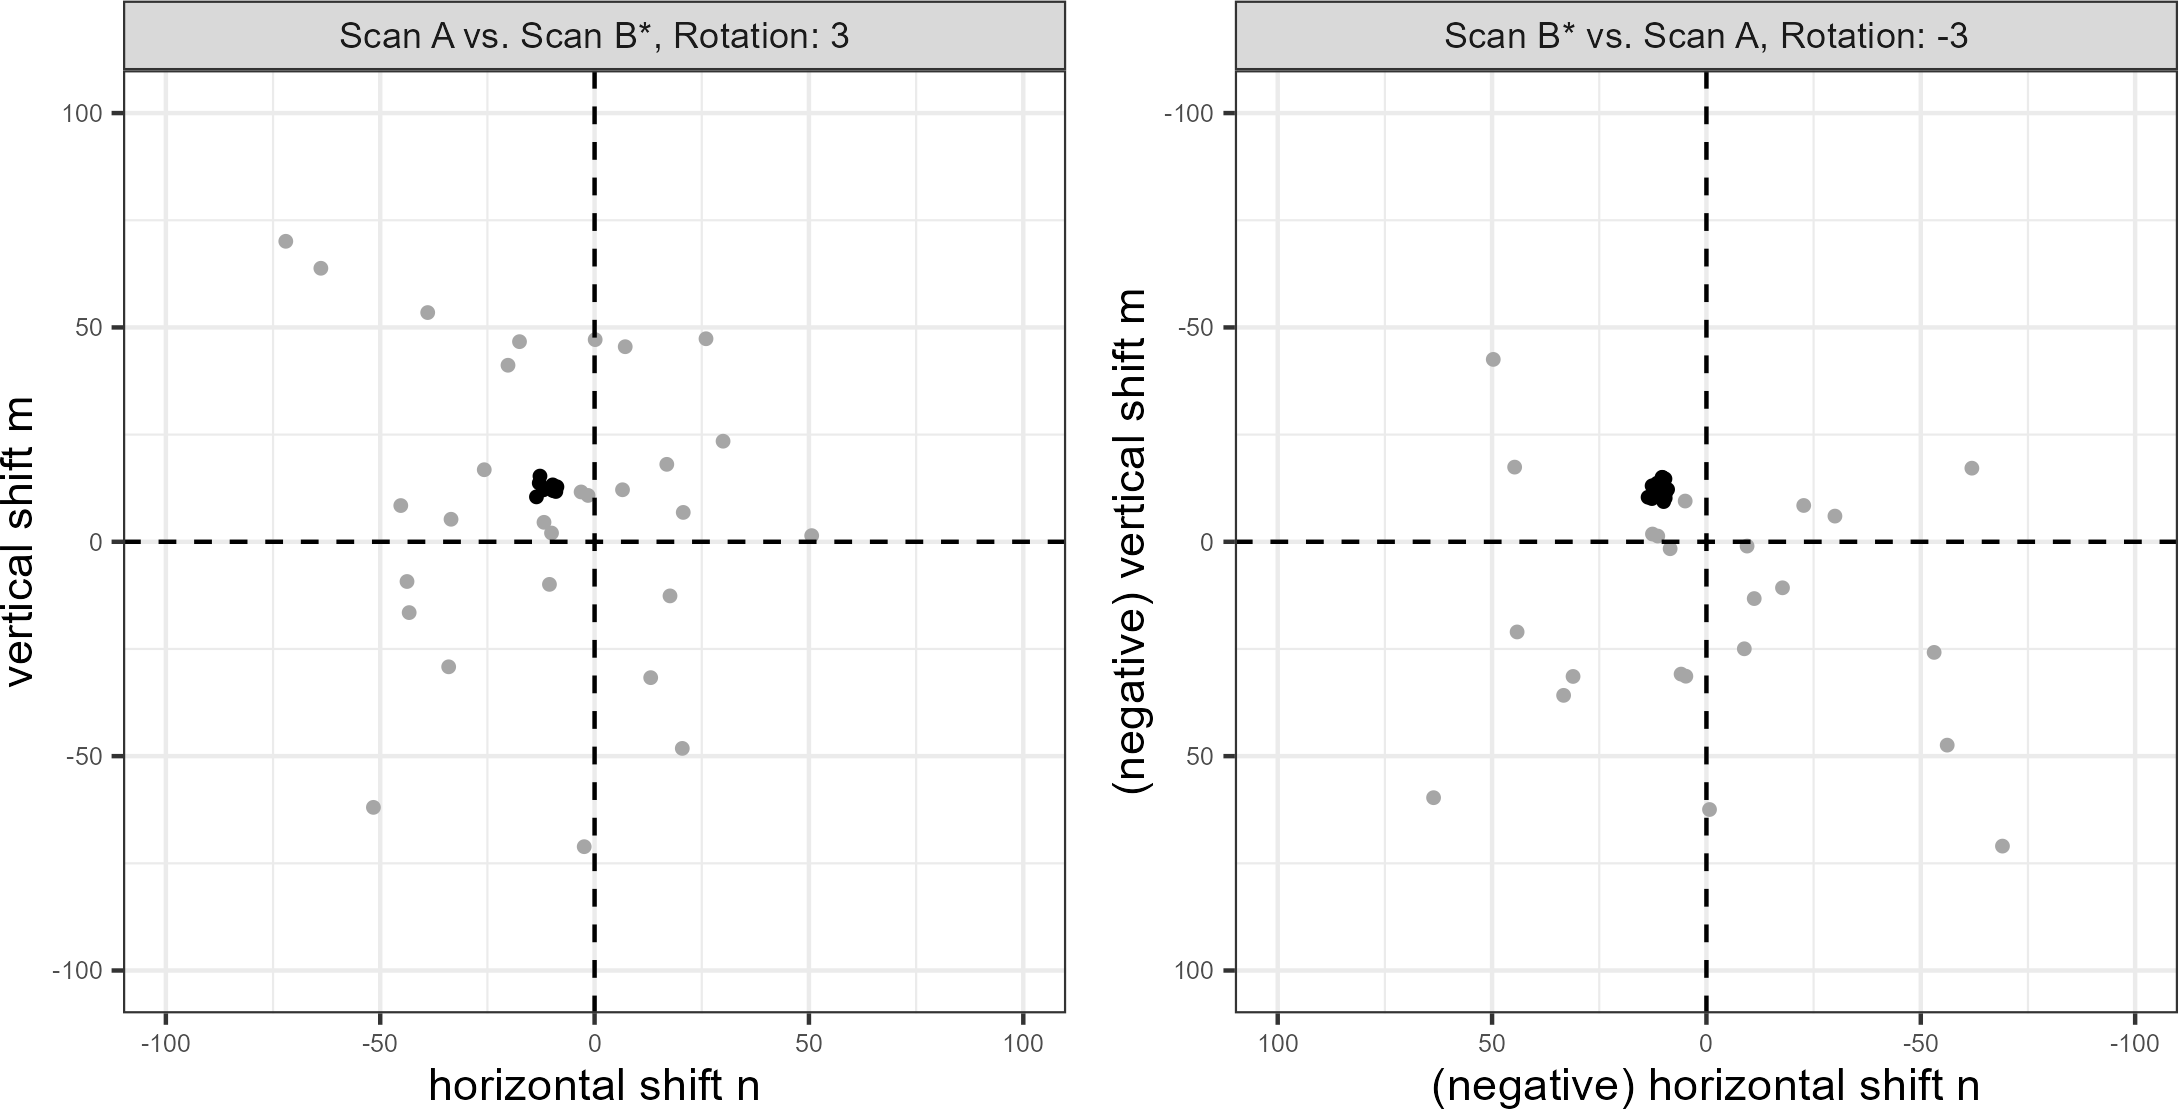
\includegraphics[width=.8\textwidth]{figures/dbscanScatterplot} 

}

\caption{\label{fig:dbscanScatterplot} Cluster assignments based on the Density Based Spatial Clustering with Applications to Noise (DBSCAN) algorithm for estimated translations in two comparison directions. Using scan $A$ as source results in a cluster of size 14 (left) compared to 13 when scan $B$ is used as source (right). Noting the reversed axes in the right plot, we see that the clusters are located approximately opposite of each other. Points are jittered for visibility.}\label{fig:unnamed-chunk-14}
\end{figure}
\end{CodeChunk}

Because \(A\) and \(B\) are truly matching, we expect the estimated
registrations in these two comparison directions to be opposites.
Indeed, the mean cluster centers in \autoref{fig:dbscanScatterplot} are
\((\hat{m}_A,\hat{n}_A,\hat{\theta}_A) \approx (16.9, -16.7, 3^\circ)\)
when \(A\) is used as source compared to
\((\hat{m}_B,\hat{n}_B,\hat{\theta}_B) \approx (-16.2, 16.8, -3^\circ)\)
when \(B^*\) is used as source.

We calculate numerical features based on the DBSCAN cluster assignments.
We first use a 2D kernel density estimator {[}cite kde2d from MASS(?){]}
to identify the rotation \(\hat{\theta}_d\) at which the per-cell
translations achieve the highest density. Next, we compute clusters
using the DBSCAN algorithm amongst the estimated translations
\(\{(m^*_{d,t,\hat{\theta}_d},n^*_{d,t,\hat{\theta}_d}) : t = 1,...,T_d\}\)
like those shown in
\autoref{fig:dbscanScatterplot}.\footnote{If more than one cluster is identified, we binarize the points based on whether they were assigned to any cluster or if they are a noise point and proceed as if there is only one cluster. We assume that two or more clusters form only because of the course rotation grid considered. Were a finer grid used, the points would coalesce into a single cluster around the true translation value. This assumption has empirical support through our experimentation.}
Let \(\pmb{C}_d\) denote the set of cells in the DBSCAN cluster. We
treat the mean cluster centers as the estimated translations
\([\hat{m}_d,\hat{n}_d]\).

We consider features related to whether a DBSCAN cluster is identified
in both comparison directions and, if such clusters are identified, the
average size of the clusters. We also compare the density-estimated
rotations and translations across the two comparison directions. These
are summarized in the \textbf{average DBSCAN cluster size}, the
\textbf{DBSCAN cluster indicator}, and the
\textbf{root squared sum of the density-estimated registrations}:
\begin{align*}
C &= \frac{1}{2}\left(|\pmb{C}_A| + |\pmb{C}_B|\right) \\
C_0 &= I(|\pmb{C}_A| > 0 \text{ and } |\pmb{C}_B| > 0)\\
\Delta_\theta &= |\hat{\theta}_A + \hat{\theta}_B| \\
\Delta_{\text{trans}} &= \sqrt{(\hat{m}_A + \hat{m}_B)^2 + (\hat{n}_A + \hat{n}_B)^2}
\end{align*} where \(|\pmb{C}_d|\) denotes the cardinality of
\(\pmb{C}_d\) and \(I(\cdot)\) is the identify function equals 1 if the
predicate argument ``\(\cdot\)'' evaluates to TRUE and 0 otherwise. We
use both \(C\) and \(C_0\) because of potential missingness in the
values of \(C\) if no cluster is identified. Missing \(C\) values are
imputed using the median non-missing value when fitting classifiers, so
the missingness information is retained in \(C_0\).

\autoref{fig:densityDistributions} shows the distributions of the
density-based features \(C\), \(\Delta_\theta\), and
\(\Delta_{\text{trans}}\). The stacked bar chart in the top-left shows
the proportion of comparisons where no DBSCAN cluster is identified by
outcome (match or non-match). We see that the vast majority of
comparisons for which no DBSCAN cluster is identified are non-match
comparisons. indicating that \(C_0\) is a good indicator of outcome. In
fact, there is only one non-match comparison that resulted in a DBSCAN
cluster. It's difficult to see in the plots, but the \(C\) value for
this non-match pair is 5 and the \(\Delta_{\text{trans}}\) value is
23.9. As expected, \(C\) tends to be relatively large for matching
comparisons while \(\Delta_{\theta}\) and \(\Delta_{\text{trans}}\)
tends to be small.

\begin{CodeChunk}
\begin{figure}[htbp]

{\centering 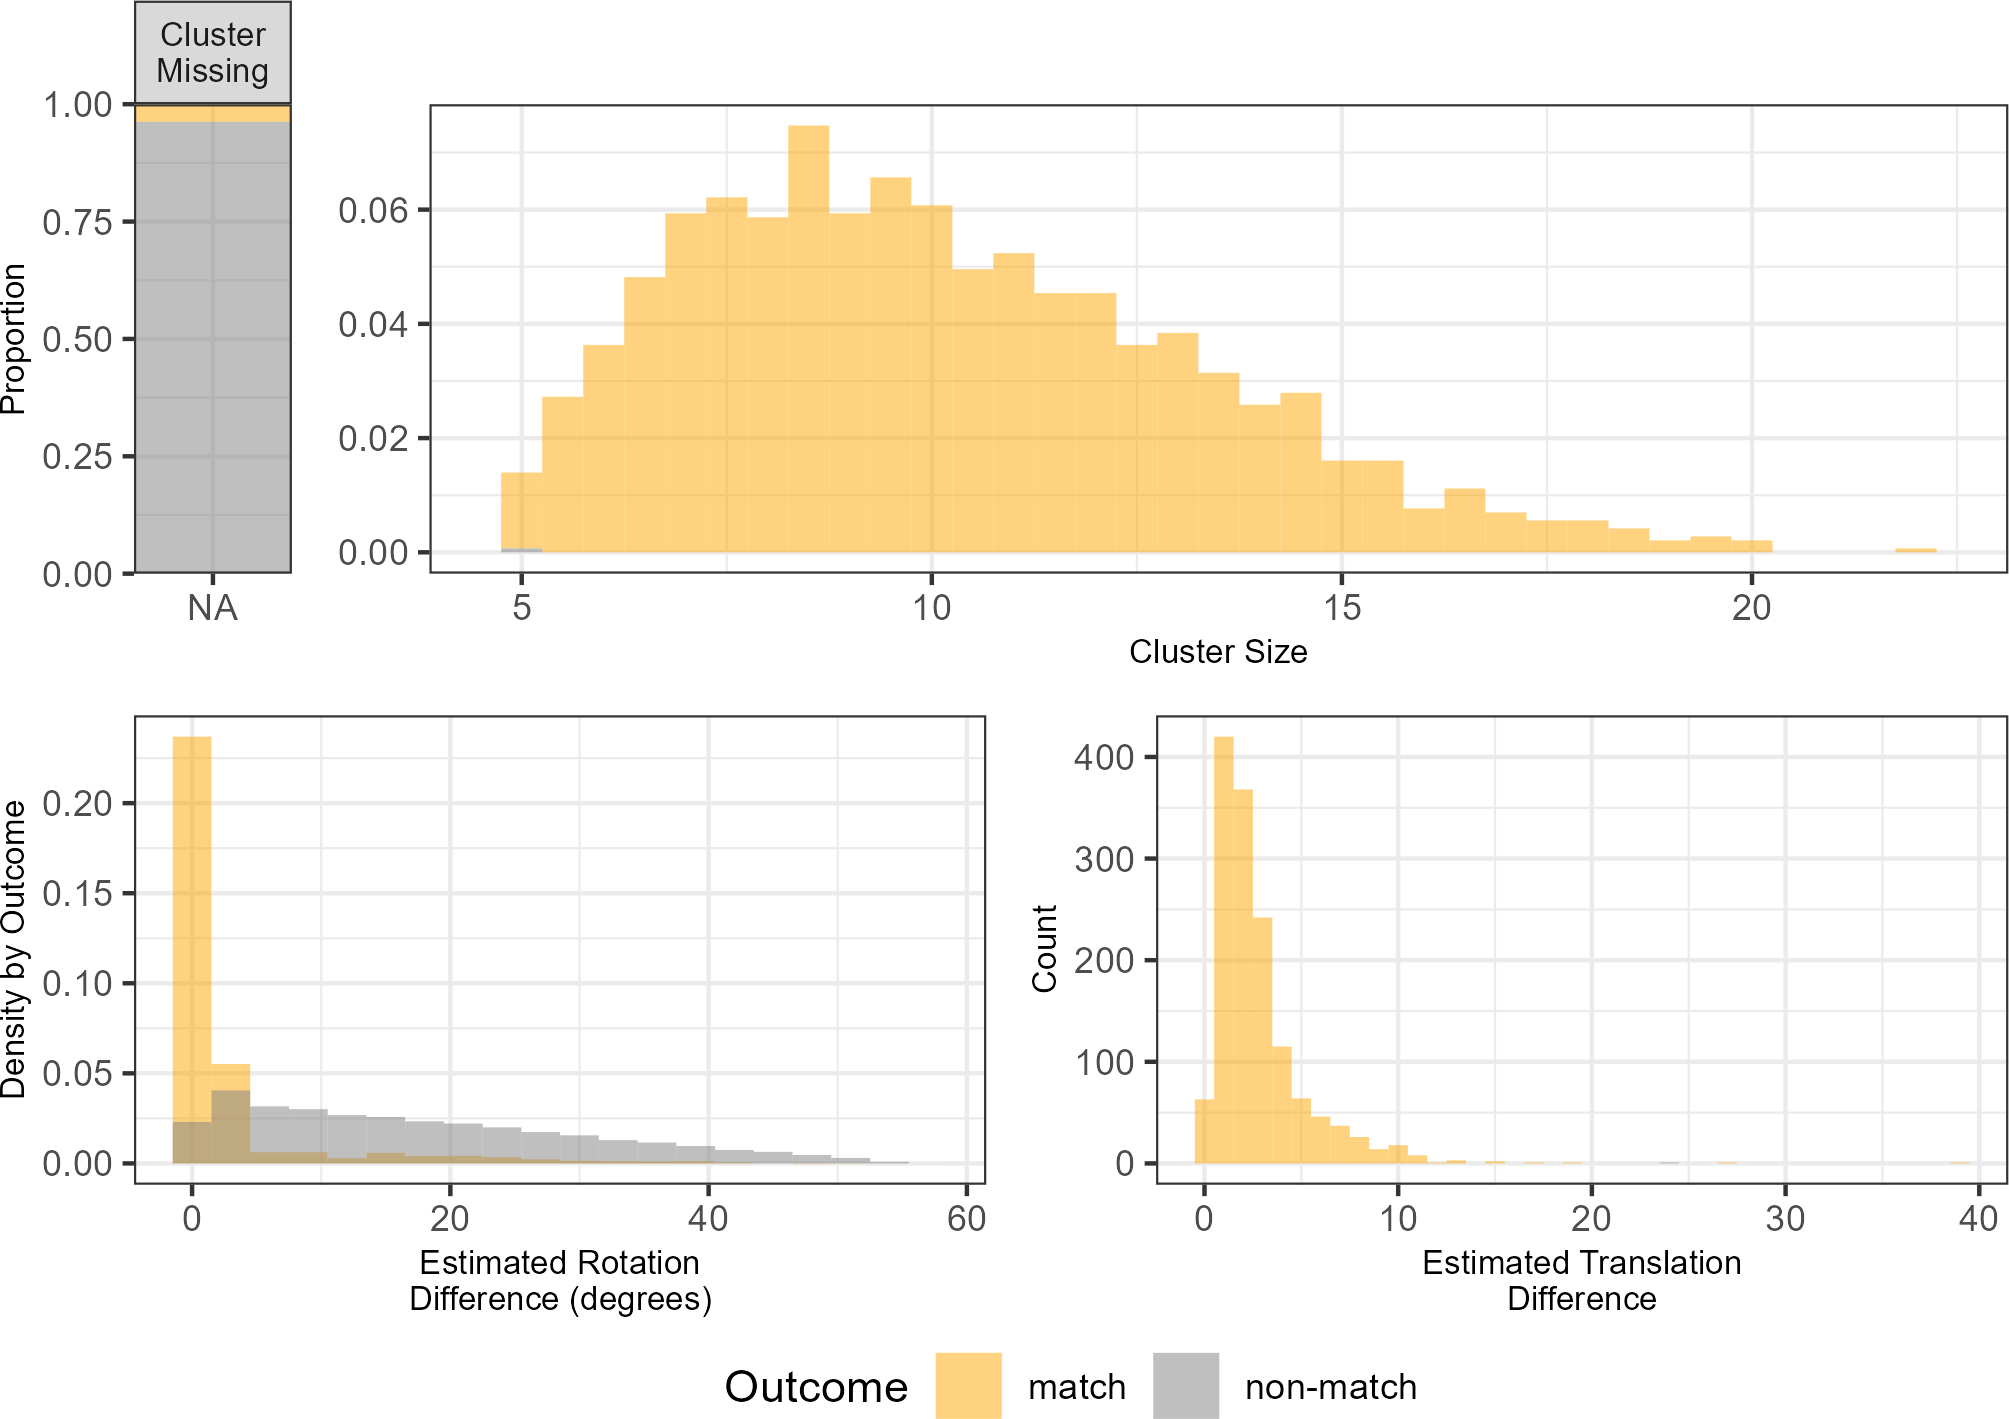
\includegraphics[width=\textwidth]{images/densityFeatureDistributions} 

}

\caption{\label{fig:densityDistributions} Distributions of the density-based features for 21,945 cartridge case pairs. The Cluster Size and Estimated Translation Difference features may be missing (\texttt{NA}) if no DBSCAN cluster is identified, which commonly occurs for non-matching cartridge case pairs as evidenced by the stacked bar chart in the top left. This explains the near absence of non-matching comparisons from Cluster Size and Estimated Translation Difference plots. Whether a cluster is identified for a particular comparison strongly predicts whether it is a match or a non-match, which justifies the inclusion of the cluster indicator feature $C_0$.}\label{fig:unnamed-chunk-15}
\end{figure}
\end{CodeChunk}

For truly matching cartridge case pairs, we expect the \(C\) to be
large, \(C_0\) to be 1, and \(\Delta_\theta, \Delta_{\text{trans}}\) to
be small. We obtain four density-based features summarized in
\autoref{tab:dbscanFeatures}.

\begin{table}[htbp]
\centering
\begin{tabular}{|p{.11\linewidth}|p{.7\linewidth}|}
\hline
Notation & Feature Description \\
\hline
$C$ & \textbf{Average DBSCAN cluster size} across both comparison directions \\
\hline
$C_0$ & \textbf{DBSCAN cluster indicator} of whether DBSCAN clusters exist in both comparison directions \\
\hline
$\Delta_\theta$ & \textbf{Absolute sum of the density-estimated rotations} between both comparison directions  \\
\hline
$\Delta_{\text{trans}}$ & \textbf{Root sum of squares of the cluster-estimated translations} between both comparison directions \\
\hline
\end{tabular}
\caption{Four similarity features based on the density-based clustering procedure.}
\label{tab:dbscanFeatures}
\end{table}

\hypertarget{visual-diagnostic-features}{%
\subsubsection{Visual Diagnostic
Features}\label{visual-diagnostic-features}}

The final set of features we calculate are based on visual diagnostic
tools described in {[}Zemmels et al.~(2023){]}. These numerical features
quantify the qualitative observations one can make from the diagnostics.

To create the visual diagnostics, we perform element-wise matrix
operations. In particular, for a matrix
\(X \in \mathbb{R}^{k \times k}\) and condition
\(cond: \mathbb{R}^{k \times k} \to \{TRUE,FALSE\}^{k \times k}\), we
define an element-wise filter operation
\(\mathcal{F}: \mathbb{R}^{k \times k} \to \mathbb{R}^{k \times k}\) as:
\begin{align*}
\mathcal{F}_{cond}(X) = 
(f_{ij})_{1 \leq i,j \leq k} =
\begin{cases}
x_{ij} &\text{if $cond$ is $TRUE$ for element $i,j$} \\
NA &\text{otherwise}
\end{cases}
\end{align*} Of particular interest in our application is the (absolute)
difference between surface matrices. For example,
\(\mathcal{F}_{|A - B| > \tau}(A)\) contains elements of matrix \(A\)
where the pair of scans \(A\) and \(B\) deviate by at least
\(\tau \in \mathbb{R}\). Surface values in \(A\) and \(B^*\) that are
``close,'' meaning within \(\tau\) distance, to each other are replaced
with \(NA\) in this filtered matrix.

The Complementary Comparison Plot visualizes the similarities and
differences between two scans. \autoref{fig:fullScan_comparisonPlot}
shows a Complementary Comparison plot between scan \(A\) and \(B^*\)
defined previously. The left column shows Scans \(A\) and \(B^*\). The
middle column shows a filtered element-wise average between \(A\) and
\(B^*\); namely
\(\mathcal{F}_{|A - B^*| < \tau}\left(\frac{1}{2}(A + B^*)\right)\).
This filtered element-wise average emphasizes similarities between \(A\)
and \(B^*\). The right column shows
\(\mathcal{F}_{|A - B^*| > \tau}(A)\) and
\(\mathcal{F}_{|A - B^*| > \tau}(B^*)\) on top and bottom, respectively.
These plots emphasize the differences between the two scans. The
complementary comparison plot is a powerful tool for assessing the
estimated alignment and identifying similarities and differences between
two surface matrices. We repeat this in the other comparison direction
\((d = B)\) to obtain filtered matrices
\(\mathcal{F}_{|A^* - B| < \tau}\left(\frac{1}{2}(A^* + B)\right)\),
\(\mathcal{F}_{|A^* - B| > \tau}(A^*)\) and
\(\mathcal{F}_{|A^* - B| > \tau}(B)\).\footnote{As with the registration-based features, in reality these matrices should be equivalent across the two comparison directions. However, there are slight differences due to the discretely-indexed nature of the surface matrices.}

\begin{CodeChunk}
\begin{figure}[htbp]

{\centering 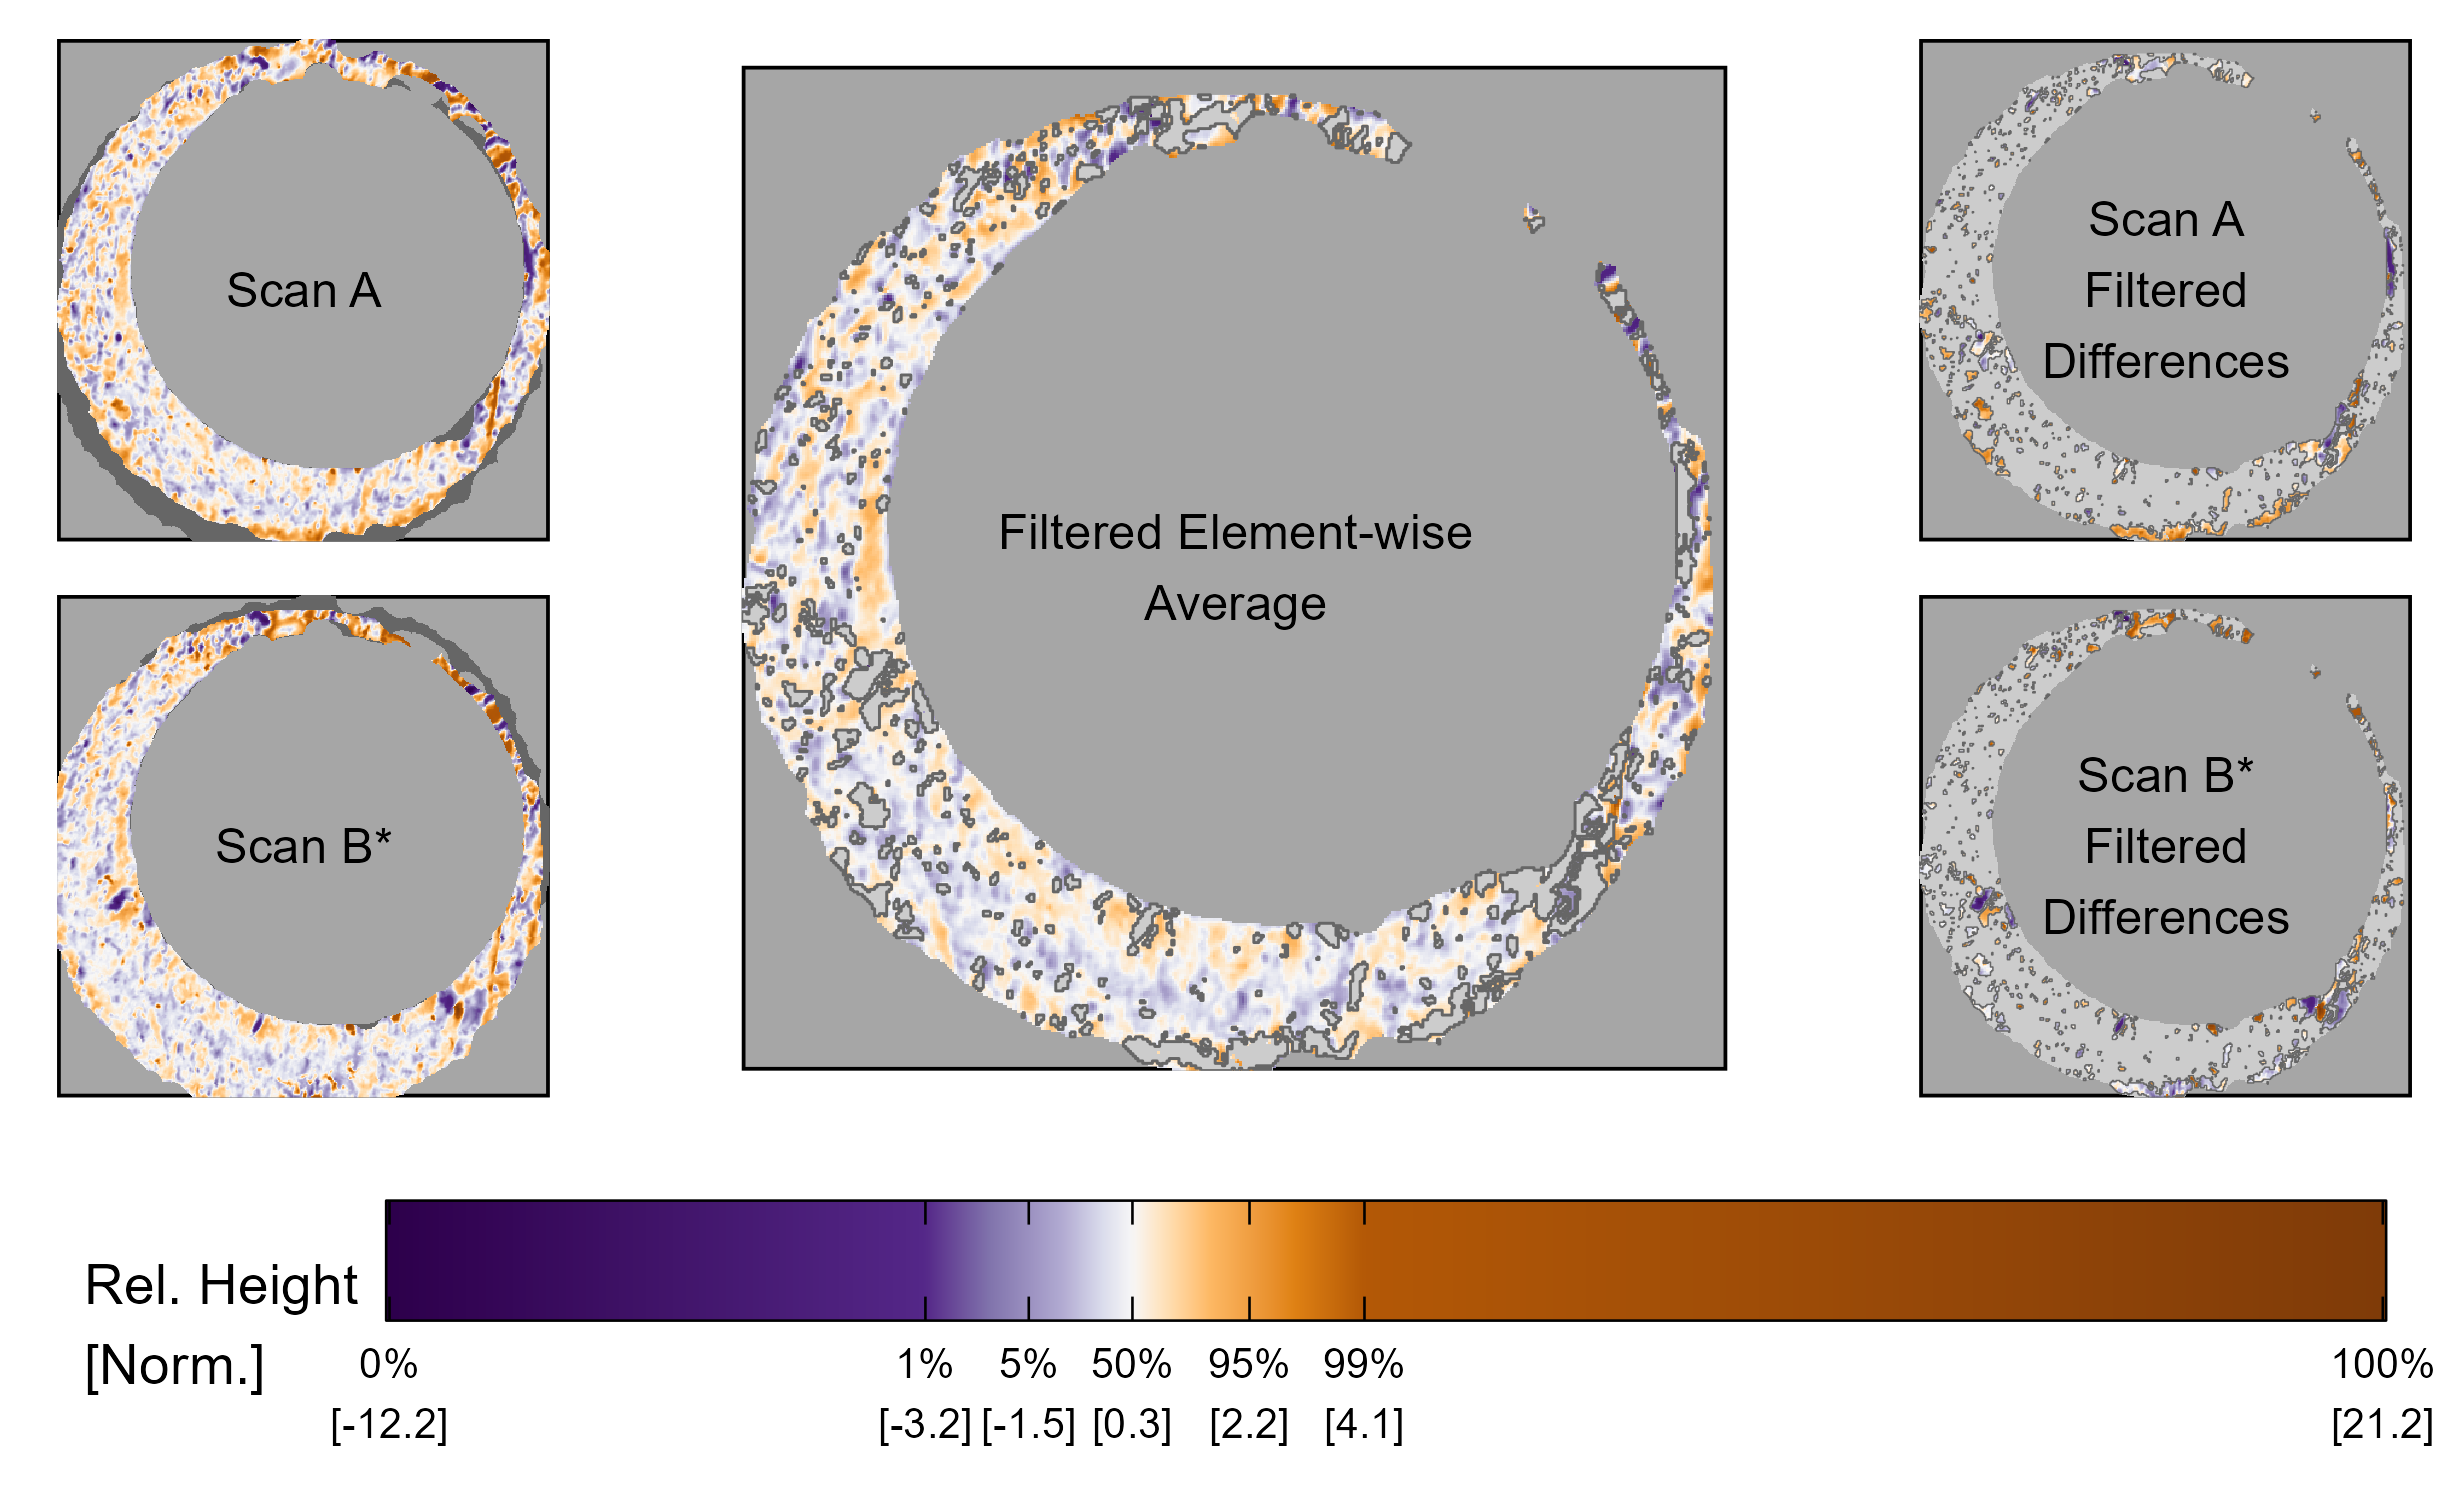
\includegraphics[width=\textwidth]{figures/fullScan_comparisonPlot} 

}

\caption{\label{fig:fullScan_comparisonPlot} Full scan comparison plot.}\label{fig:unnamed-chunk-19}
\end{figure}
\end{CodeChunk}

We make a series of qualitative assumptions related to how a
Complementary Comparison Plot will look for matching and non-matching
cartridge case pairs. We develop a set of features that measure the
degree to which these assumptions are met by a particular cartridge case
pair. We now describe each feature and their associated assumptions.

We first consider the correlation \(cor_{d,\text{full},\text{filt}}\)
between the filtered matrices \(\mathcal{F}_{|A - B^*| > \tau}(A)\) and
\(\mathcal{F}_{|A - B^*| > \tau}(B^*)\) when \(d = A\) and
\(\mathcal{F}_{|A^* - B| > \tau}(A^*)\) and
\(\mathcal{F}_{|A^* - B| > \tau}(B)\) when \(d = B\). The average of
these is used as a feature: \begin{align*}
\overline{cor}_{\text{full},\text{filt}} = \frac{1}{2}\left(cor_{A,\text{full},\text{filt}} + cor_{B,\text{full},\text{filt}}\right).
\end{align*} We assume that
\textbf{average filtered full-scan pairwise-complete correlation} will
be larger for truly matching \(A\) and \(B\) than non-matching. Said
another way, we assume that even surface regions of \(A\) and \(B\) that
are different will follow similar trends, which can occur due to
variability in the amount of contact between a cartridge case and breech
face across multiple fires of a single firearm. The correlation is
calculated by vectorizing the two filtered surface matrices and treating
missing values by case-wise deletion.

As before, we extend this notation to accommodate cell comparisons
\(t = 1,...,T_d\) for \(d = A,B\) using subscripts:
\(cor_{d,t,\text{filt}}\). For example, \(cor_{A,t,\text{filt}}\) is the
correlation between cell filtered surface matrices
\(\mathcal{F}_{|A_t - B_{t,\theta_t^*}^*| > \tau}(A_t)\) and
\(\mathcal{F}_{|A_t - B_{t,\theta_t^*}^*| > \tau}(B_{t,\theta_t^*}^*)\)
where \(B_{t,\theta_t^*}^*\) is the matrix extracted from \(B^*\) that
maximizes the CCF with \(A_t\). We calculate the sample mean of the
filtered correlation values across all cells and both directions:
\begin{align*}
\overline{cor}_{\text{cell},\text{filt}} &= \frac{1}{T_A + T_B} \sum_{d \in \{A,B\}} \sum_{t=1}^{T_d} cor_{d,t,\text{filt}}
\end{align*}

Next, we consider features based on the elements of the Boolean \(cond\)
matrix. Consider \autoref{fig:filterLabeling} that shows the filtered
element-wise average
\(\mathcal{F}_{|A - B^*| < \tau}\left(\frac{1}{2}(A + B^*)\right)\) on
the left and the associated \(cond\) matrix \(|A - B^*| < \tau\)
visualized in black-and-white in the middle where filtered elements are
shown in white. We use a connected components labeling algorithm
detailed in {[}Haralick and Shapiro (1992){]} to identify individual
neighborhoods of filtered elements. More precisely, the algorithm
returns a set of sets \(\pmb{S}_d = \{S_{d,1},S_{d,2},...,S_{d,L_d}\}\)
where each \(S_{d,l}\) is a set of indices of the \(cond\) matrix that
have a value of \(TRUE\) and are connected by a chained-together
sequence of 4 (Rook's) neighborhoods. The right side of
\autoref{fig:filterLabeling} shows each \(S_{d,l}\) distinguished by
different fill colors, \(l = 1,...,L_d\).

\begin{CodeChunk}
\begin{figure}[htbp]

{\centering 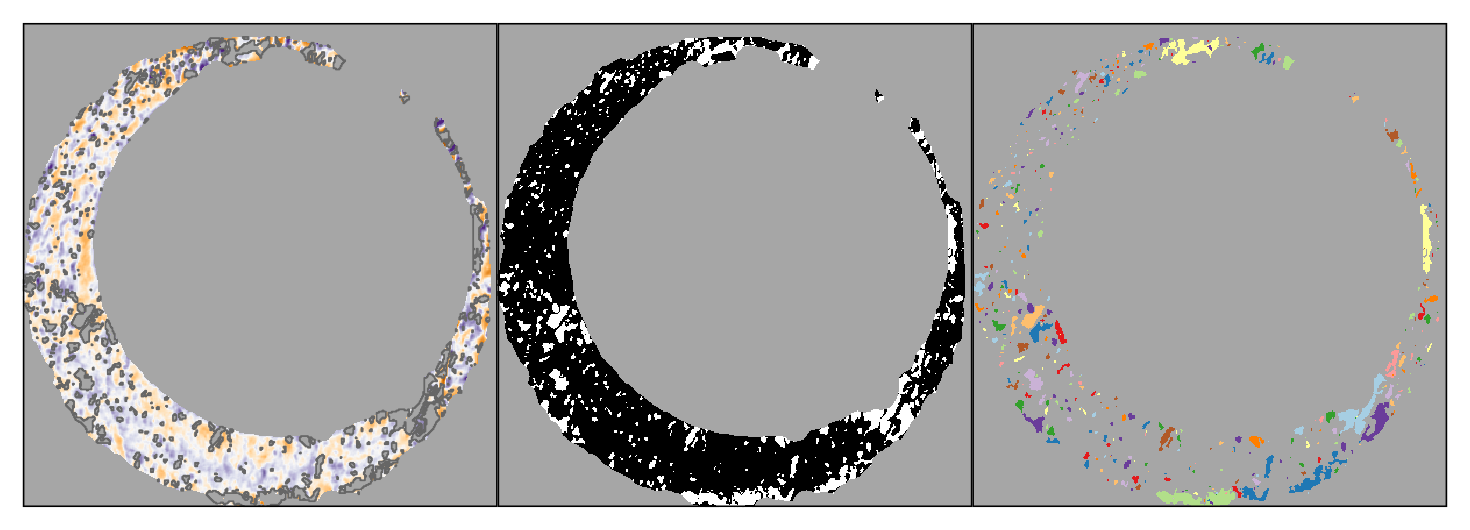
\includegraphics[width=\textwidth]{figures/filterLabeling} 

}

\caption{\label{fig:filterLabeling} (Left) After aligning two scans, we filter regions that are "different" from each other, meaning the absolute difference between surface values is larger than some threshold. (Middle) We binarize the scan into "filtered" or "non-filtered" regions - shown in white and black, respectively. (Right) Using a connected components labeling algorithm, we identify connected "neighborhoods" of filtered elements. We assume that these neighborhoods will be small, on average, if comparing truly matching cartridge cases.}\label{fig:unnamed-chunk-22}
\end{figure}
\end{CodeChunk}

We calculate the following features using the full-scan labeled
neighborhoods: \begin{align*}
\overline{|S|}_{\text{full}} &= \frac{1}{L_A + L_B} \sum_{d \in \{A,B\}} \sum_{l=1}^{L_d} |S_{d,l}| \\
s_{\text{full},|S|} &= \sqrt{\frac{1}{L_A + L_B - 1} \sum_{d \in \{A,B\}} \sum_{l=1}^{L_d} (|S_{d,l}| - \overline{|S|}_{\text{full}})^2}
\end{align*} where \(|S_{d,l}|\) is the size of the set \(S_{d,l}\). We
assume that the \textbf{average} and
\textbf{standard deviation of the filtered full-scan neighborhood sizes}
will be small for truly matching cartridge cases. That is to say, we
assume that the the surface regions of \(A\) and \(B\) that are
different will all be small, on average, and vary little in size. This
assumption is appropriate assuming that the breech face leaves
consistent markings on fired cartridge cases.

Again, we extend the notation to accommodate individual cells. Let
\(\pmb{S}_{d,t} = \{S_{d,t,1},...,S_{d,t,L_{d,t}}\}\) denote the set of
labeled neighborhoods for a cell \(t = 1,...,T_d\), \(d = A,B\). We
calculate the per-cell average and standard deviation of the labeled
neighborhood cell size: \begin{align*}
\overline{|S|}_{d,t} &= \frac{1}{L_{d,t}} \sum_{l=1}^L |S_{d,t,l}| \\
s_{d,t,|S|} &= \sqrt{\frac{1}{L_{d,t} - 1} \sum_{l=1}^{L_{d,t}} (|S_{d,t,l}| - \overline{|S|}_{\text{cell},d,t})^2}.
\end{align*}

We assume that the cell-based \(\overline{|S|}_{d,t}\) and
\(s^2_{d,t,|S|}\) will be small, on average, for truly matching
cartridge cases. Consequently, we use the sample average of these as
features: \begin{align*}
\overline{|S|}_{\text{cell}} &= \frac{1}{T_A + T_B} \sum_{d \in \{A,B\}} \sum_{t=1}^{T_d} \overline{|S|}_{d,t} \\
\bar{s}_{\text{cell},|S|} &= \frac{1}{T_A + T_B} \sum_{d \in \{A,B\}} \sum_{t=1}^{T_d} s_{d,t,|S|}
\end{align*} Again, we assume that the
\textbf{average cell-wise neighborhood size} and the
\textbf{average standard deviation of the cell-wise neighborhood sizes}
will be small for truly matching cartridge cases.

\autoref{fig:visualDiagnosticDensities} shows the distribution of the
six visual diagnostic-based features. As expected, matching comparisons
at the full-scan and cell-based levels tend to have smaller neighborhood
sizes and higher correlation values on average.

\begin{CodeChunk}
\begin{figure}[htbp]

{\centering 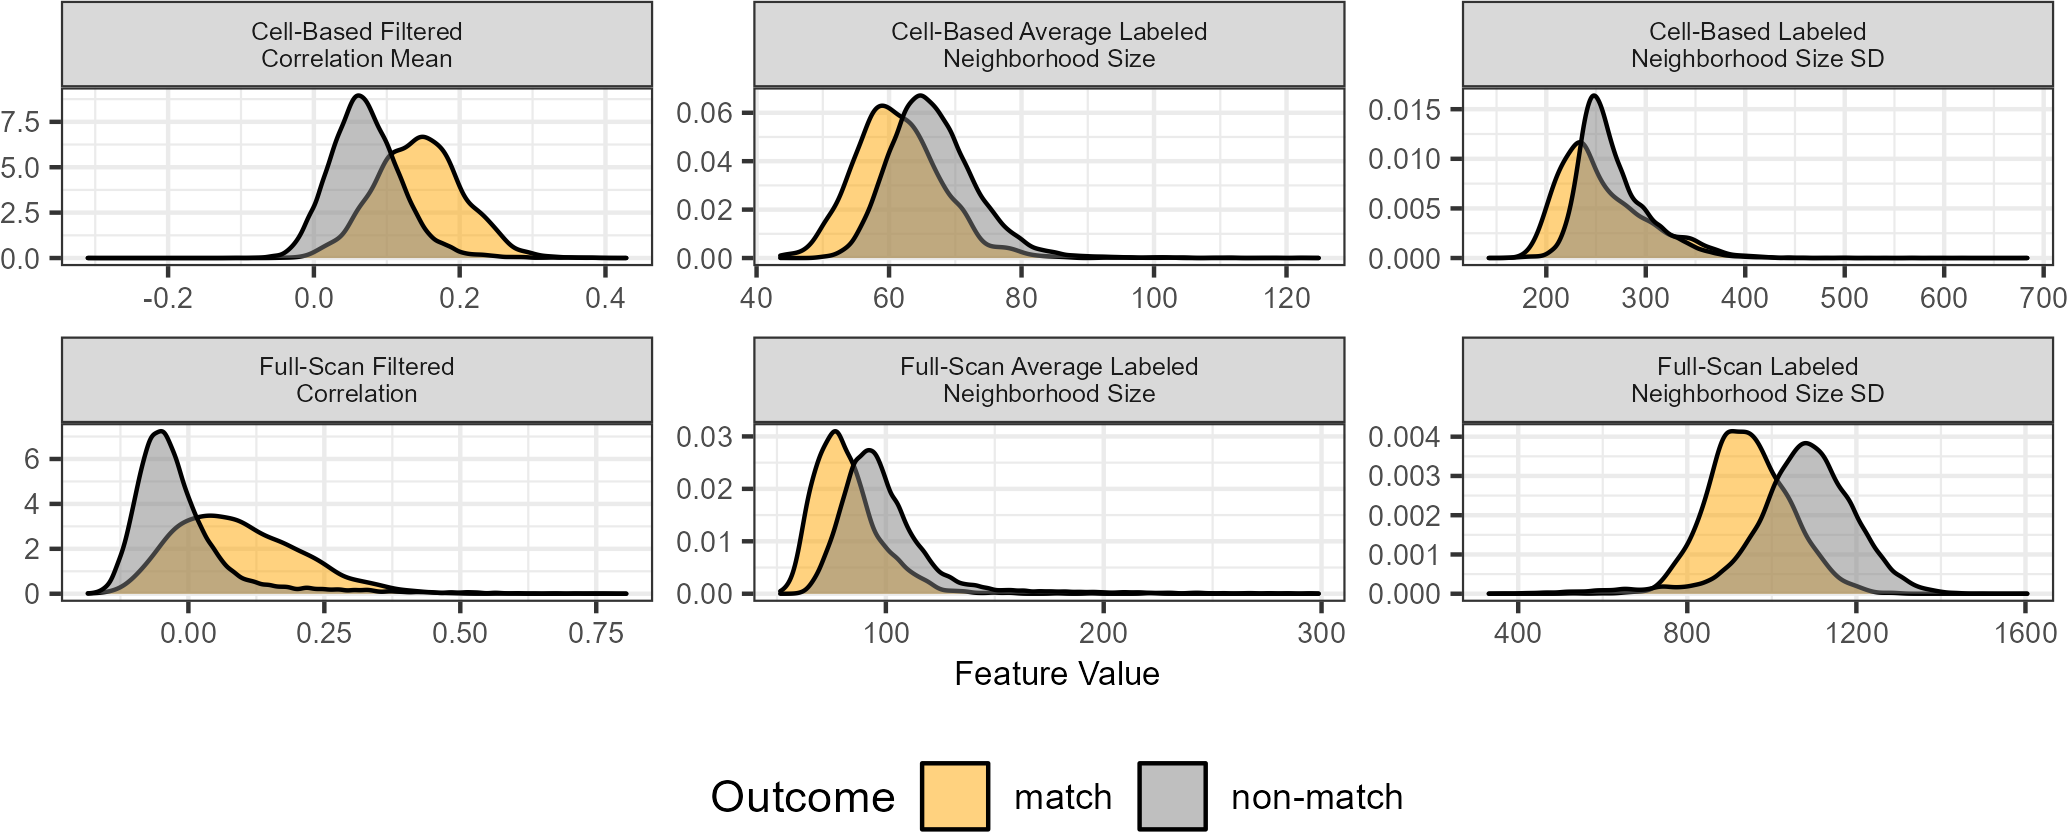
\includegraphics[width=\textwidth]{images/visualDiagnosticDensities} 

}

\caption{\label{fig:visualDiagnosticDensities} Distributions of the visual diagnostic-based features for 21,945 cartridge case pairs. Matching comparisons tend to have smaller neighborhood sizes on average and higher correlation values than non-matches indicating their utility in a classifier.}\label{fig:unnamed-chunk-23}
\end{figure}
\end{CodeChunk}

\autoref{tab:visualDiagnosticFeatures} summarizes the 7 features
calculated based on the visual diagnostics.

\begin{table}[htbp]
\centering
\begin{tabular}{|p{.11\linewidth}|p{.7\linewidth}|}
\hline
Notation & Feature Description \\
\hline
$\overline{cor}_{\text{full},\text{filt}}$ & \textbf{Average filtered full-scan correlation} across both comparison directions \\
\hline
$\overline{cor}_{\text{cell},\text{filt}}$ & \textbf{Average filtered cell-wise correlation} across all cells in both comparison directions \\
\hline
$\overline{|S|}_{\text{full}}$ & \textbf{Average filtered full-scan neighborhood size} across both comparison directions \\
\hline
$s_{\text{full},|S|}$ & \textbf{Standard deviation of the filtered full-scan neighborhood sizes} across both comparison directions \\
\hline
$\overline{|S|}_{\text{cell}}$ & \textbf{Average filtered cell-wise neighborhood sizes} across all cells in both comparison directions \\
\hline
$\bar{s}_{\text{cell},|S|}$ & \textbf{Average standard deviation of the cell-wise neighborhood sizes} across all cells in both comparison direction \\
\hline
\end{tabular}
\caption{Seven similarity features calculated based on visual diagnostics.}
\label{tab:visualDiagnosticFeatures}
\end{table}

\hypertarget{scoring}{%
\subsection{Scoring}\label{scoring}}

We randomly split the cartridge case data set into 10 barrels for
training and 15 barrels for testing. Multiple cartridge cases were fired
from each barrel, so this resulted in a training data set of 210
cartridge cases, \(\binom{210}{2} = 21,945\) pairwise comparisons, and a
testing set of 300 cartridge cases, \(\binom{300}{2} = 44,850\) pairwise
comparisons.

We perform 10-fold cross-validation to train binary classifiers. We
compare the results of three classifiers: based on a logistic
regression, a Classification and Regression Tree (CART) model, and a
random forest \citep{R,rpart,randomForest,caret}.

{[}Write full logistic regression model here{]}

We consider the pros and cons of each of these models. The logistic
regression and CART models are more interpretable than a random forest
yet, as we will see, a random forest tends to be more accurate. The
following section detail the results of this cross-validation procedure.

\hypertarget{results}{%
\section{Results}\label{results}}

\hypertarget{training-results}{%
\subsection{Training Results}\label{training-results}}

\autoref{fig:trainingAccuracy} shows the cross-validation estimated
accuracies for the three trained models. We consider the performance of
the three models under different subsets of the ACES feature set, which
provides insight into the importance of the various feature groups. We
see that the random forest trained on the full ACES data set results in
the highest overall accuracy of \(98.9\%\). For each feature group, the
the random forest yields the highest accuracy followed by the logistic
regression and CART models. We see that the removing the cluster-based
features has a notable impact on the accuracy of the logistic regression
and CART models, while the random forest is more is more robust.

\begin{CodeChunk}
\begin{figure}[htbp]

{\centering 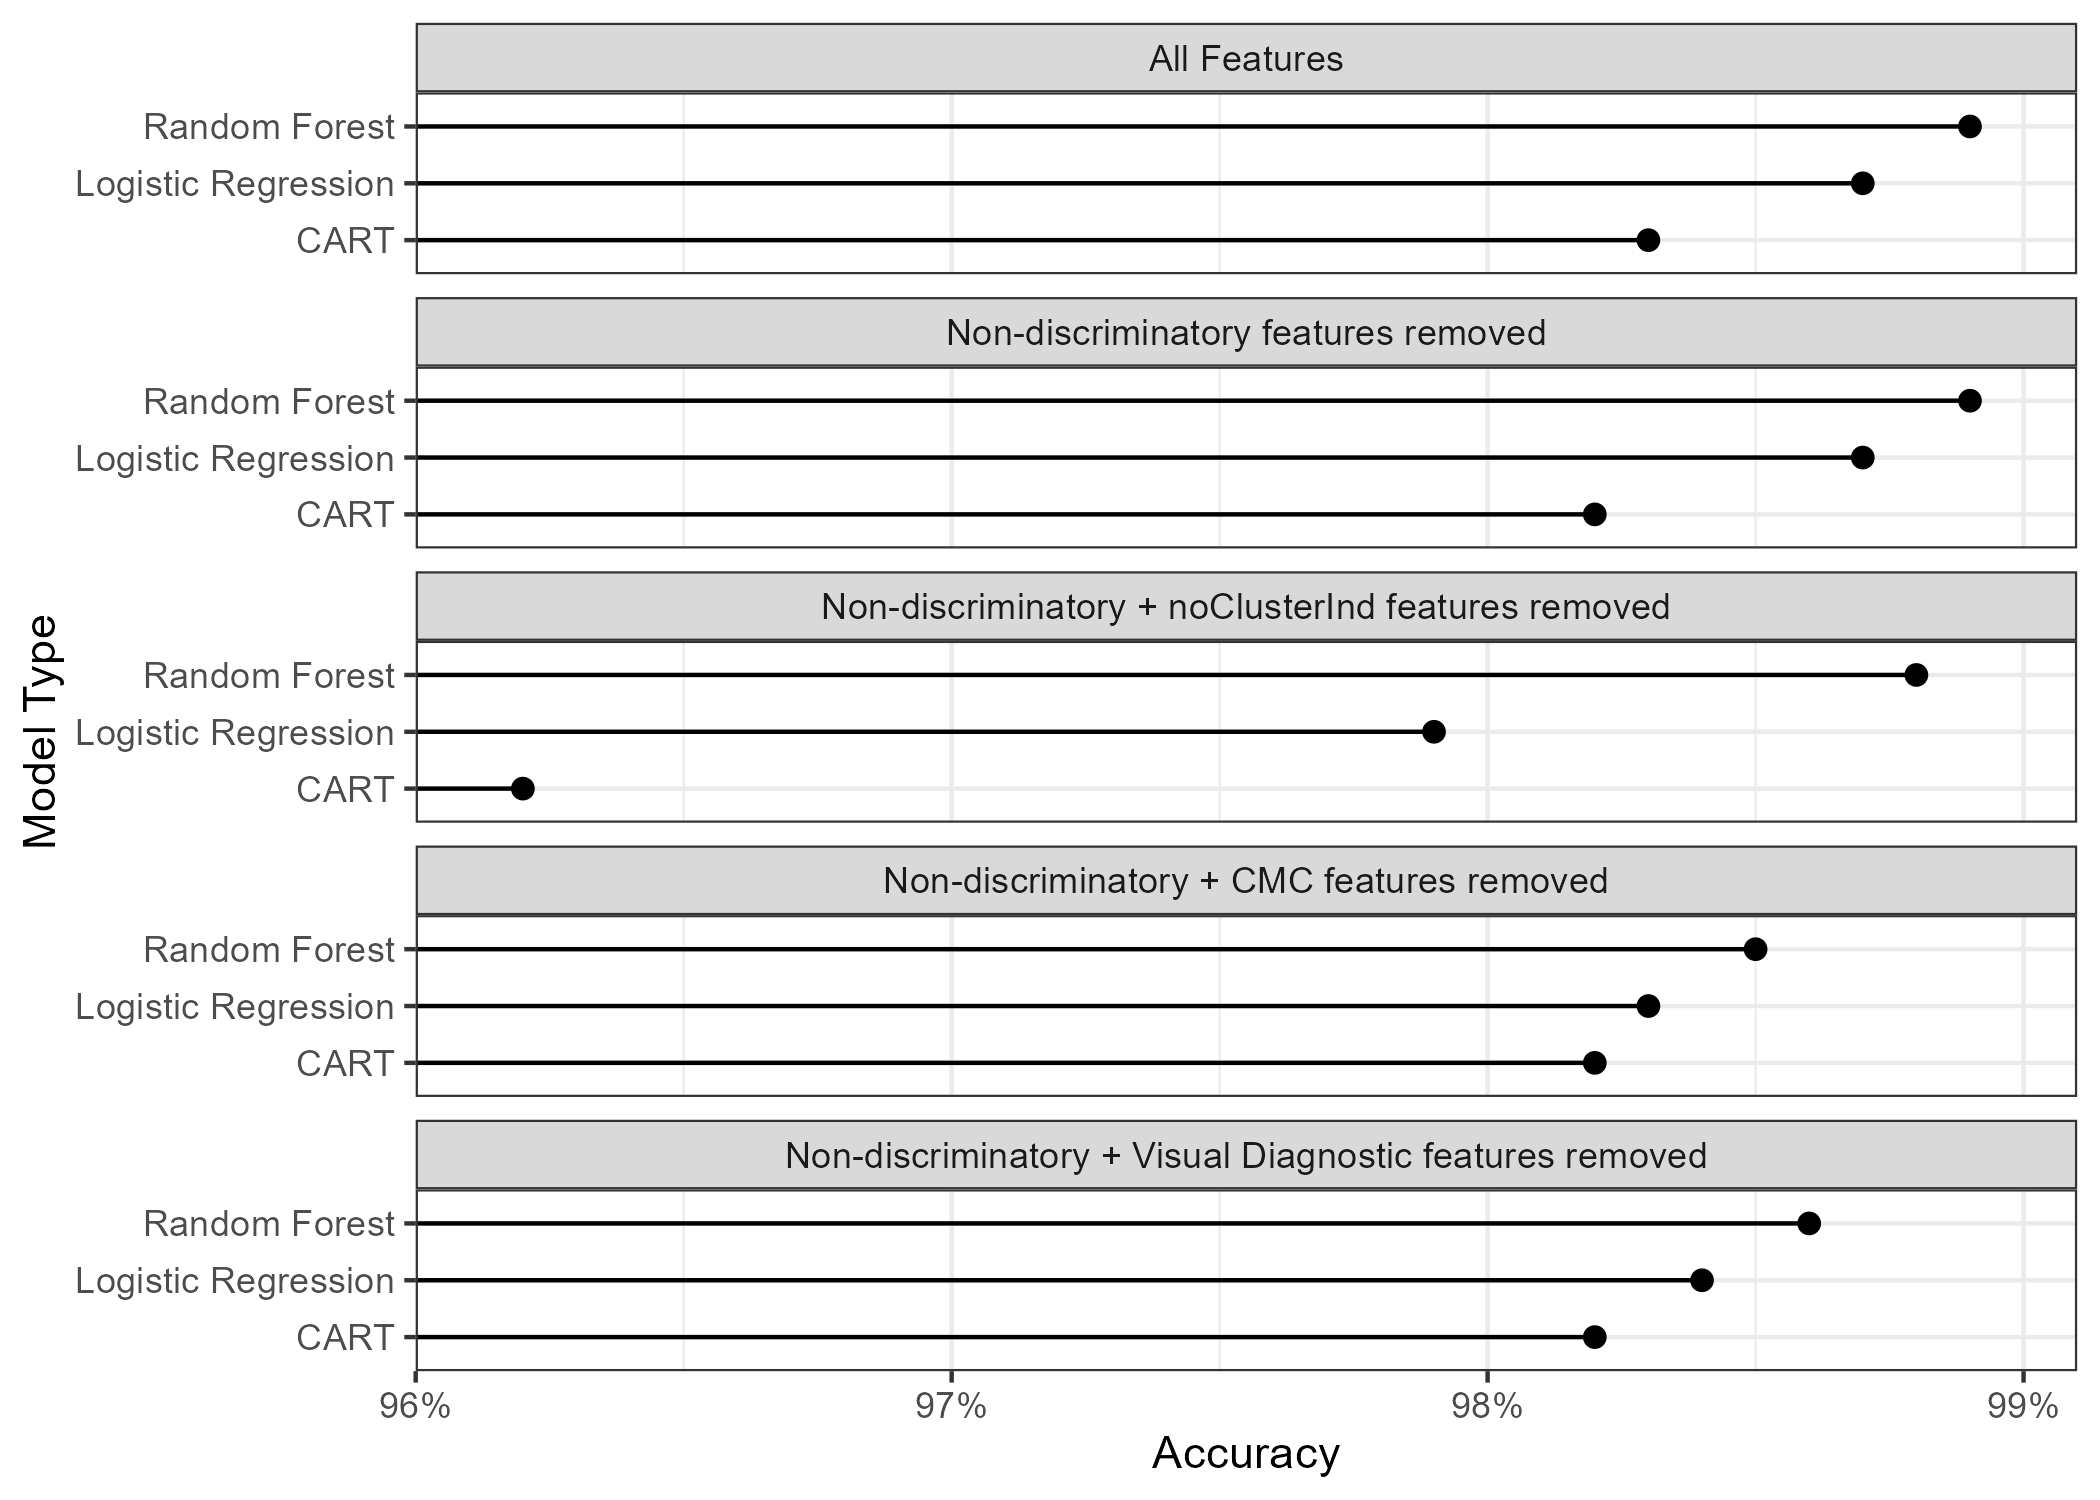
\includegraphics[width=.8\textwidth]{figures/trainingAccuracy} 

}

\caption{\label{fig:trainingAccuracy} Training classification accuracy for random forest (RF), logistic  regression (LR), and classification and regression tree (CART) models based on various subsets of the training data set features. These accuracies are estimated based on 10-fold cross validation repeated thrice. In general, the Classification and Regression Tree (CART) model performs poorest while the Random Forest performs best. Removing the cluster-based features has the largest impact on the accuracies.}\label{fig:unnamed-chunk-25}
\end{figure}
\end{CodeChunk}

\begin{CodeChunk}
\begin{figure}[htbp]

{\centering 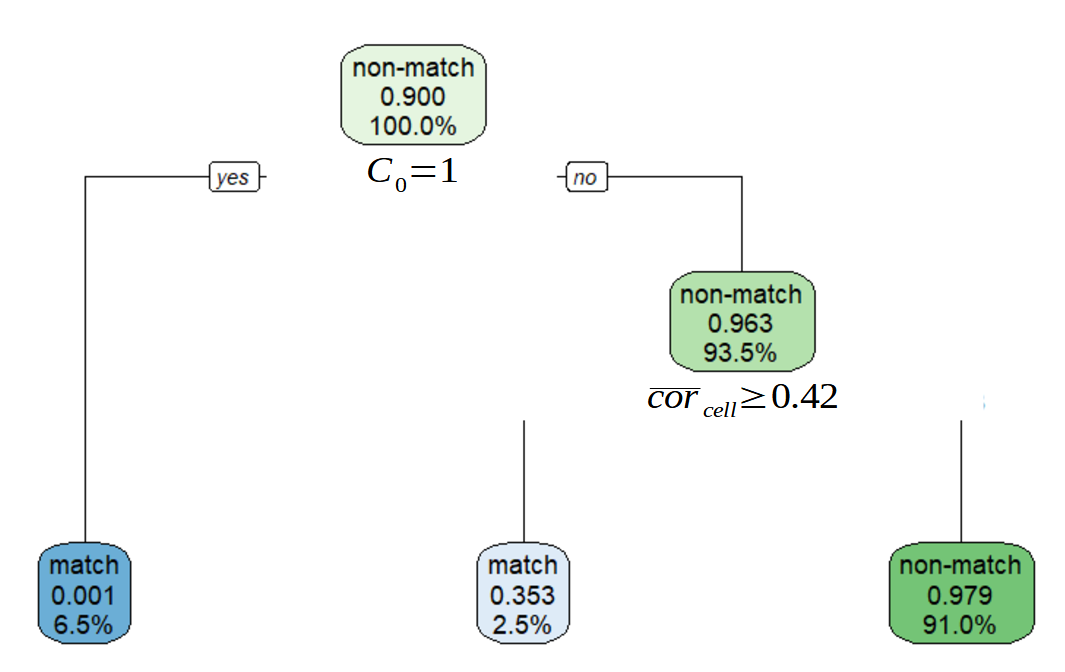
\includegraphics[width=\textwidth]{images/trainedCART_labeled} 

}

\caption{\label{fig:trainedCART} Trained Classification and Regression Tree model.}\label{fig:unnamed-chunk-26}
\end{figure}
\end{CodeChunk}

\autoref{fig:rfVarImpPlt} shows the distribution of a variable
importance measure for each feature across fittings of a random forest
model using 10 random seeds. For each replicate, we measure a variable's
importance using the Gini Index, which measures the probability of
making a misclassification for a given model {[}cite Gini Index
resource{]}. {[}More exposition on Gini Index?{]} Noting the log scale
on which these points are plotted, we see that the ``no cluster
indicator'' variable is considered by far the most important variable
across the random forest fittings. The ``cell-based pairwise-complete
correlation'' and ``cluster size'' are also important, although it's
less clear which is more important due to their distributional overlap.
Overall, the results indicate that the cluster-based aggregation and
cell-based registration features are considered most important by the
random forest models.

\begin{CodeChunk}
\begin{figure}[htbp]

{\centering 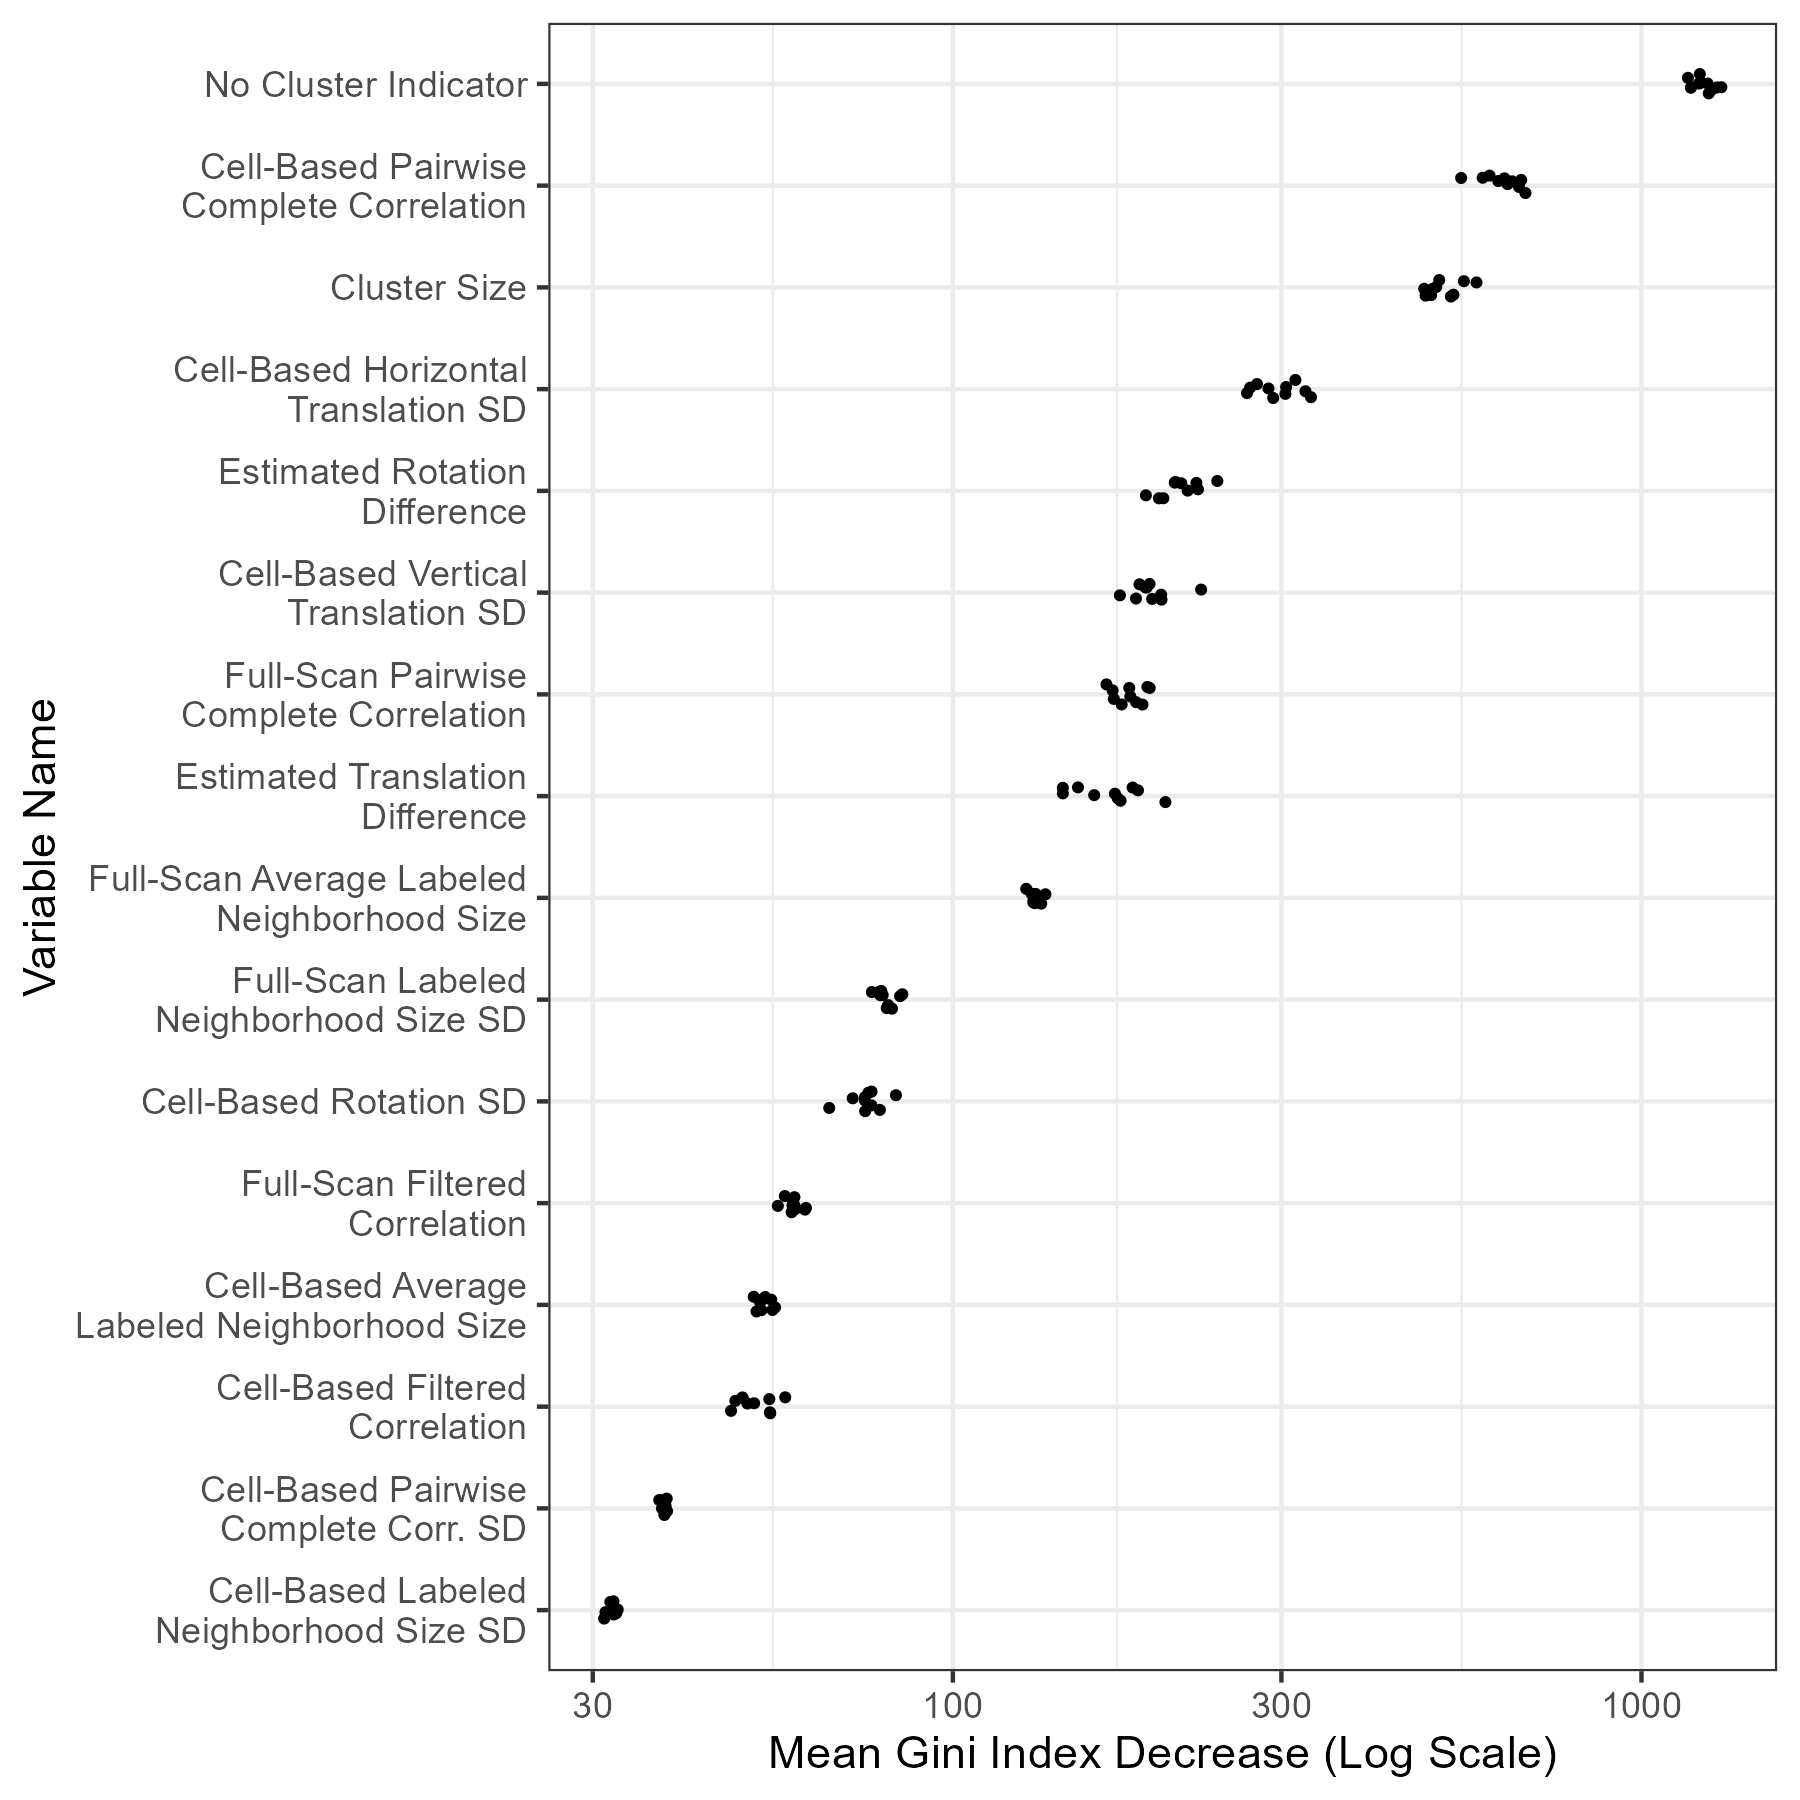
\includegraphics[width=4in,height=4in]{figures/varImportanceBoxplot} 

}

\caption{\label{fig:rfVarImpPlt} Variable importance measures from fitting a random forest to the training data set, repeated 10 times under various random seeds. Points are plotted on a log scale and vertically jittered for visibility. The No Cluster Indicator feature is by far the most important feature, as measured by the mean decrease in the Gini index.}\label{fig:unnamed-chunk-28}
\end{figure}
\end{CodeChunk}

\hypertarget{testing-results}{%
\subsection{Testing Results}\label{testing-results}}

For each of the 44,850 cartridge case pairs in the testing data set, we
use each model to predict whether the pair is a match or non-match. An
error occurs when this prediction does not match the ground-truth nature
of the cartridge case pair. \autoref{fig:testingAccuracy} summarizes the
error rates for each method. The Accuracy is the overall percentage of
correct classifications. The True Negative rate is percentage of
correctly-classified non-match pairs. Conversely, the True Positive rate
is the percentage of correctly-classified matching pairs.

We see that the testing accuracy across models and feature groups is
similar to that of the training results in
\autoref{fig:trainingAccuracy}. The random forest is more robust to
changes in feature group while the CART model performs uniformly worse
than the other models. Interestingly, the logistic regression model
performs slightly better than the random forest for some feature groups.
Considering the true positive and negative rates, this can be explained
by the specificity of the models: the logistic regression model
classifies non-matches more effectively in these instances, although
this difference is slight.

\begin{CodeChunk}
\begin{figure}

{\centering 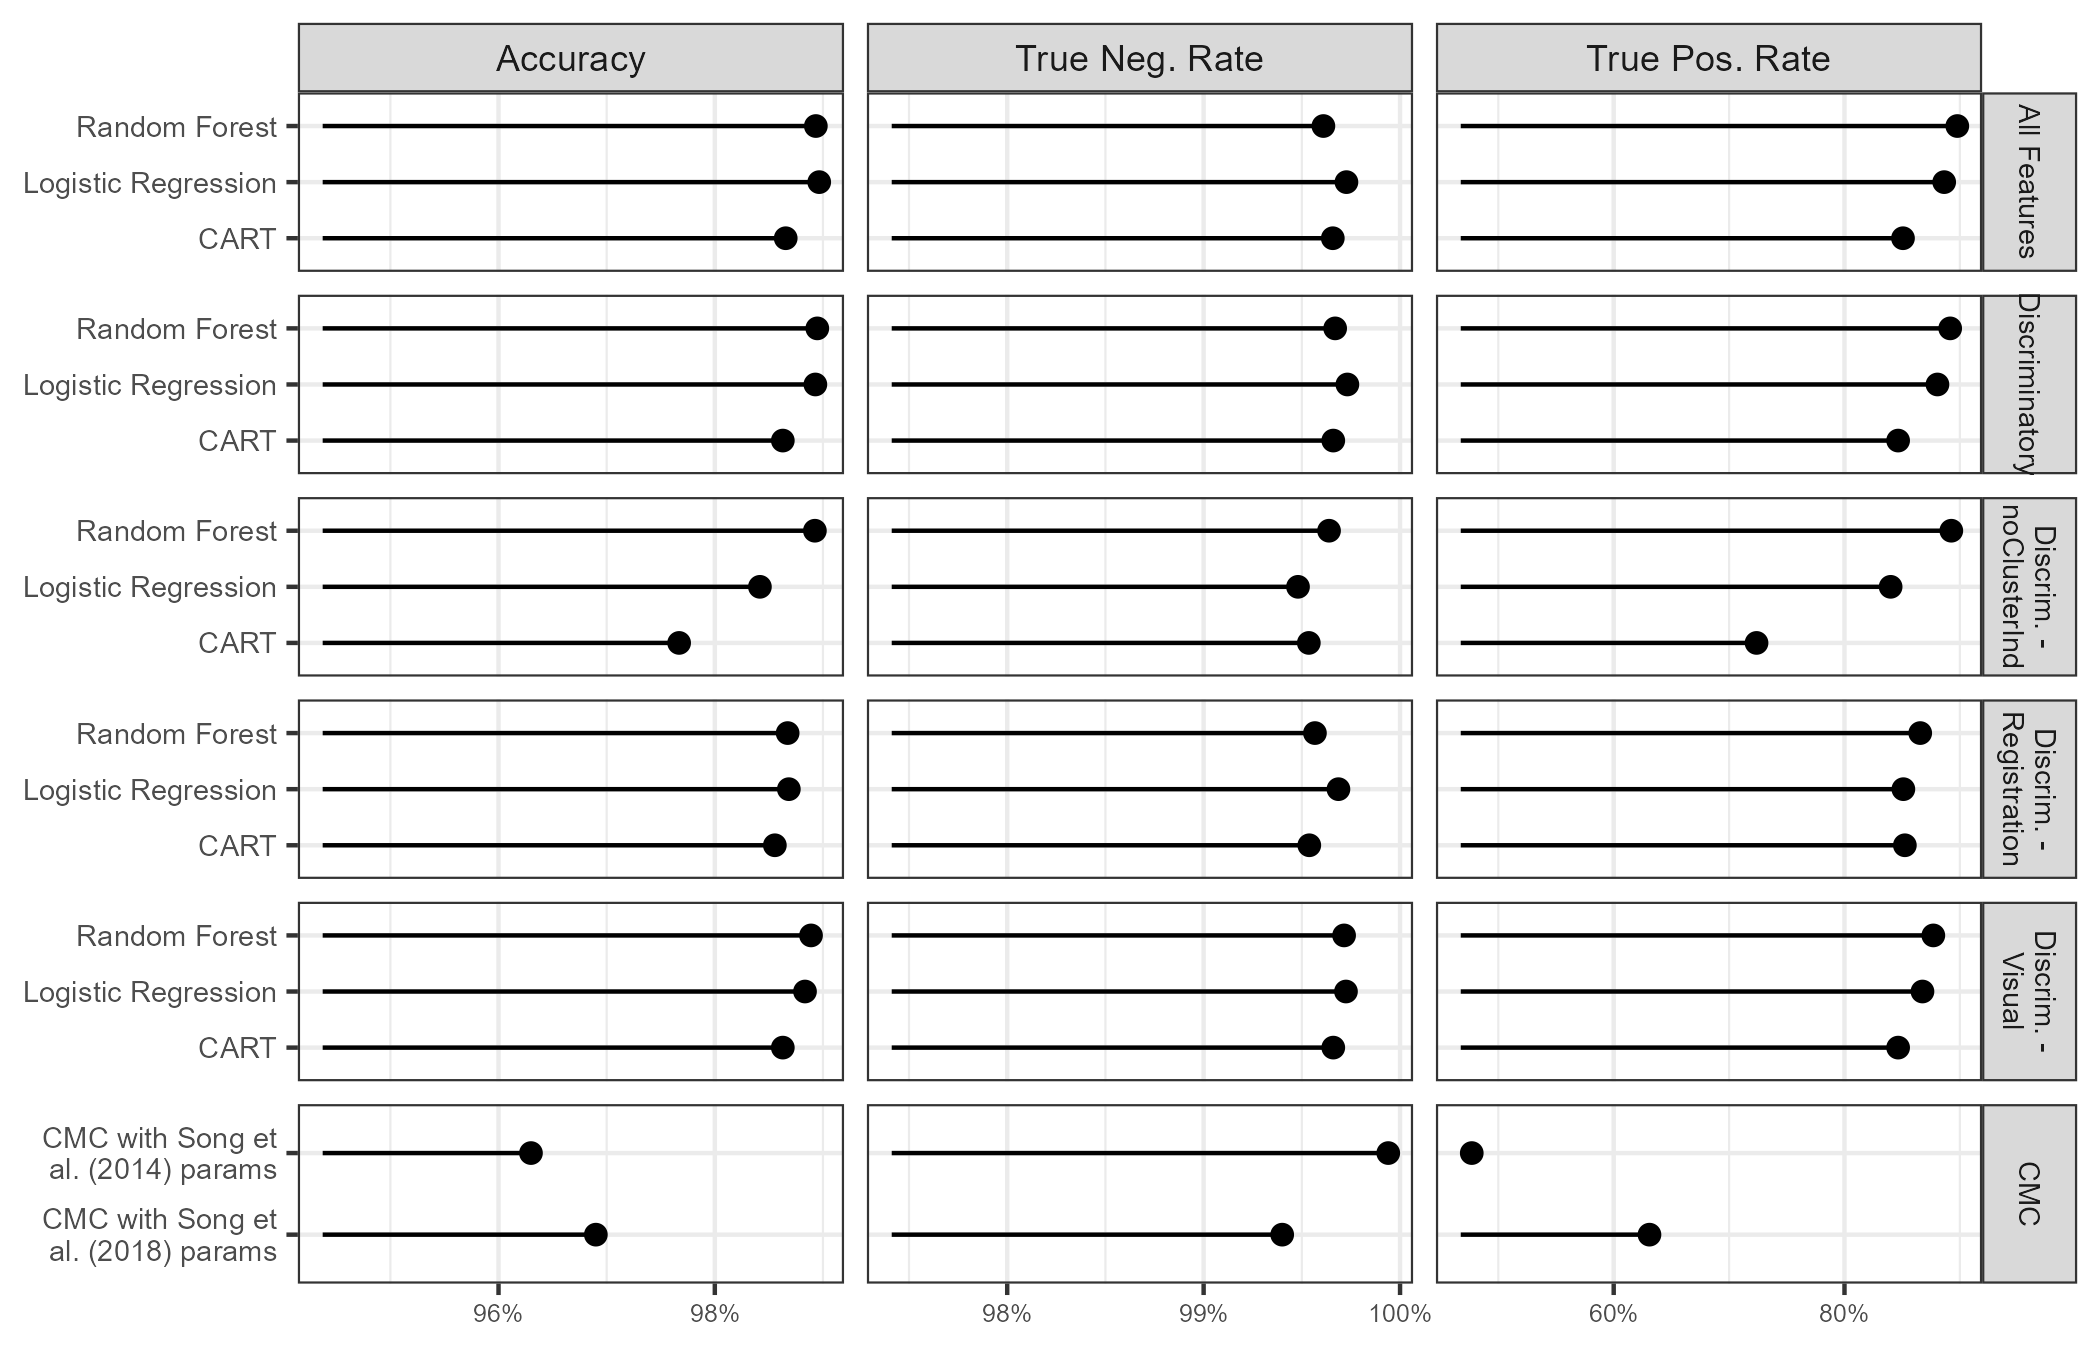
\includegraphics[width=\textwidth]{figures/testAccuracy} 

}

\caption{\label{fig:testingAccuracy} Testing classification accuracy, false negative rate, and false positive rate faceted by various subsets of the testing data set features. The Logistic Regression model performs about as well as the Random Forest model in classifying matches and non-matches amongst the test data set. This is primarily because the Logistic Regression model is has a higher true negative rate while the Random Forest model has a higher true positive rate. The CART model lags behind in the three metrics.}\label{fig:unnamed-chunk-30}
\end{figure}
\end{CodeChunk}

\hypertarget{discussion}{%
\section{Discussion}\label{discussion}}

\hypertarget{comparing-classifier-models}{%
\subsection{Comparing Classifier
Models}\label{comparing-classifier-models}}

Our intention in fitting different classification models was to compare
each model's strengths and weaknesses. As indicated by
\autoref{fig:testingAccuracy}, the random forest have similar testing
accuracies with the random forest being more robust to changes in
feature group. In particular, the random forest model is better at
identifying truly matching cartridge cases than the logistic regression
classifier, yet worse at identifying non-matches.

Pragmatically, it seems reasonable to choose the model with the highest
estimated accuracy. Ethically however, we might favor the model that
makes the fewest false positive classifications since mis-classifying a
truly non-matching cartridge case pair may incriminate an innocent
individual. While the input of statisticians is important, this decision
needs to be weighed by the wider forensic and legal communities.

While the random forest is generally more accurate, the CART and
logistic regression models are more interpretable. For example, as seen
in {[}figure{]}, the CART model provides a set of simple, binary rules
by which we can arrive at a classification. {[}More on CART? Perhaps
compare a single decision tree to random forest?{]}

The estimated coefficients in the logistic regression model help us
understand the effect that each feature has on the odds that a cartridge
case pair matches. {[}Table{]} shows the multiplicative change in the
odds that a cartridge case pair matches for a one unit increase in each
feature.

Discuss benefits of three models here

\begin{itemize}
\item
  CART model is a clear set of binary ``rules'' that lead to a
  classification
\item
  Logistic Regression provides estimate of how odds of match change with
  a one unit increase of each feature
\item
  It also performs similar to the random forest
\item
  Random Forest seems to be more robust to changes
\end{itemize}

\hypertarget{comparison-to-previous-work}{%
\subsection{Comparison to Previous
Work}\label{comparison-to-previous-work}}

Our results corroborate the conclusions made in previous papers.
{[}Zhang et al.~(2020){]} proposed a binary classifier using the DBSCAN
algorithm: if a cluster is identified, then classify the cartridge case
pair as a match and otherwise a non-match. This is analogous to defining
a classification rule based solely on the ACES feature \(C_0\). Given
the importance of \(C_0\) indicated in \autoref{fig:rfVarImpPlt}, our
results indicate that a classifier based on \(C_0\) would have a
reasonably high accuracy. However, information about the size and
location of clusters in a classifier adds important nuance as indicated
by the ranking of \(\Delta_{\theta}\), \(\Delta_{\text{trans}}\), and
\(C\) in \autoref{fig:rfVarImpPlt}. For example, although one non-match
pair in the training data was assigned a DBSCAN cluster, this pair's
estimated translation difference, \(\Delta_{\text{trans}}\), was
relatively large. The ACES logistic regression and random forest models
correctly classify this pair as a non-match.

Cells identified by a DBSCAN cluster could be considered an alternative
definition of a ``Congruent Matching Cell'' (CMC) as defined in {[}Song
(2013){]}. While the intention behind the CMC method and the
density-based ACES features is the same, that is to determine the number
of cells that ``agree'' on a registration value, the manner in which
agreement is measured differs. In the original CMC algorithm, a cell is
called a CMC if its estimated registration is within some threshold of a
reference value, typically the median registration across all cells. The
registration thresholds are set manually in most CMC papers except for
{[}Zemmels et al.~(2022){]} where they are selected based on an
optimization criterion. As discussed in {[}Zemmels et al.~(2022){]}, the
CMC algorithm is quite sensitive to the choice of thresholds as well as
to noisiness in the cell-based registrations. In the ACES algorithm, we
measure agreement by the number of cells that are close to each other -
a reference value is not required, but is a byproduct of the DBSCAN
algorithm (e.g., treating cluster centroids as the estimated
translations). Further, we simplify optimization by defining
``closeness'' through the single \(\epsilon\) parameter of the DBSCAN
algorithm instead of three threshold parameters (horizontal/vertical
translation and rotation) in the CMC algorithm.

{[}Song (2013){]} measures the similarity between two cartridge cases
using the total number of CMCs and proposes classifying a pair as
matching if the CMC count exceeds five. Considering the DBSCAN cluster
size \(C\) as analogous to the CMC count, a decision boundary for \(C\)
equal to five seems reasonable; especially in light of the distribution
of \(C\) shown in \autoref{fig:densityDistributions}. Similarly,
reasonable matching registration cutoffs based on
\autoref{fig:densityDistributions} are \(3^\circ\) for rotation and 10
pixels for translation. These are similar to manually-selected
thresholds used across various CMC papers {[}Tong et al.~(2015), Chen et
al.~(2017){]}.

{[}Compare results to our best CMC method (and Baldwin?).{]}

The ACES algorithm simultaneously substantiates the classification rules
used by previously proposed cartridge case comparison algorithms while
also infusing their logic with additional nuance.

\hypertarget{conclusion}{%
\section{Conclusion}\label{conclusion}}

More experimentation is needed. It is reasonable to assume that the
version of ACES discussed in this paper would be effective at
classifying cartridge cases of the same brand, fired from the same
make/model of firearm, and scanned using the same topographical scanner
{[}cite TopMatch{]}. It remains to be seen whether the fitted models
generalize to other types of ammunition or firearm.

The train/test procedure outlined in this manuscript should be adopted
by any future researchers to validate proposed methods. {[}Discuss
availability of data and code{]}

Nonetheless, this paper provides the largest study of automatic
cartridge case comparison algorithms published to-date. Our results
indicate that there exist effective, robust, and interpretable automatic
classifiers for cartridge case evidence.

We expect the ACES feature set to evolve over time; for discriminatory
features to replace less informative features. We stress
interpretability as a guiding principle for future feature engineering.
Ideally, forensic practitioners will eventually use such algorithms to
supplement their expert opinion. We believe it paramount that
practitioners understand and can explain, at least at a high level, to a
jury of lay people the features used for classification. {[}More on why
this is important{]}

\newpage

\hypertarget{computational-details}{%
\section*{Computational Details}\label{computational-details}}
\addcontentsline{toc}{section}{Computational Details}

If necessary or useful, information about certain computational details
such as version numbers, operating systems, or compilers could be
included in an unnumbered section. Also, auxiliary packages (say, for
visualizations, maps, tables, \dots) that are not cited in the main text
can be credited here.

The results in this paper were obtained using
\proglang{R}\textasciitilde3.5.1. \proglang{R} itself and all packages
used are available from the Comprehensive \proglang{R} Archive Network
(CRAN) at \url{https://CRAN.R-project.org/}.

\hypertarget{acknowledgments}{%
\section*{Acknowledgments}\label{acknowledgments}}
\addcontentsline{toc}{section}{Acknowledgments}

All acknowledgments should be collected in this unnumbered section
before the references. It may contain the usual information about
funding and feedback from colleagues/reviewers/etc. Furthermore,
information such as relative contributions of the authors may be added
here (if any).

\bibliography{refs}

\newpage

\setcounter{section}{0}
\renewcommand{\thesection}{\Alph{section}}




\end{document}
